\documentclass{whutmod}
\usepackage{metalogo}
\usepackage{enumitem}
\usepackage{graphicx}
\usepackage{subfigure}
\usepackage {mathtools}
  
\usepackage{algpseudocode}  
\usepackage{float}
\usepackage{listings}
\usepackage{color}
\usepackage{algorithm}
\usepackage{algorithmicx}


\usepackage{amsmath}%添加矩阵宏包
\graphicspath{{figures/}} %图片在当前目录下的figures还有目录picture下,还可以继续添加其他搜索路径
\definecolor{dkgreen}{rgb}{0,0.6,0}
\definecolor{gray}{rgb}{0.5,0.5,0.5}
\definecolor{mauve}{rgb}{0.58,0,0.82}
\definecolor{backcolour}{rgb}{0.95,0.95,0.95}
\lstset{frame=tb,
	language=Python,
	backgroundcolor=\color{backcolour},   
	aboveskip=3mm,
	belowskip=3mm,
	showstringspaces=false,
	columns=flexible,
	basicstyle={\small\ttfamily},
	numbers=none,
	numberstyle=\tiny\color{gray},
	keywordstyle=\color{blue},
	commentstyle=\color{dkgreen},
	stringstyle=\color{mauve},
	breaklines=true,
	breakatwhitespace=true,
	tabsize=3
}
%插入参考文献命令
\newcommand{\upcite}[1]{\textsuperscript{\textsuperscript{\cite{#1}}}}

\renewcommand{\algorithmicrequire}{\textbf{Input:}}  % Use Input in the format of Algorithm  
\renewcommand{\algorithmicensure}{\textbf{Output:}} % Use Output in the format of Algorithm  
\team{26}	% 组号
\membera{xxx}
\joba{xxx}
\memberb{xxx}
\jobb{xxx}
\memberc{xxx}
\jobc{xxx}
\title{基于非稳态热传导的相变低温作业防护服装设计}
\tihao{1} % 题号

\begin{document}
\maketitle
\begin{abstract}
	本文通过分析超低温环境下相变材料的放热特点和防护服系统热传导原理,建立了基于非稳态热传导方程的相变低温作业防护服装设计模型,对该环境下不同体质和新陈代谢状态的工作者提出了合理的防护服设计方案。
		
	针对问题一,本文建立了基于\textbf{非稳态热传导}的偏微分方程模型,对防寒服热量传递情况进行仿真,求解了工作者低温作业的安全时间。该模型对防寒服人体系统构建了\textbf{皮肤-空气间隔-内层-中间层-最外层5层热量传导面},主要考虑了热传导及热对流两种热传递方式,利用\textbf{Fourier热传导定理},确定了防寒服各层接触面的衔接条件和介质内的控制方程。利用\textbf{牛顿冷却定律},确定了外界环境与服装系统的热对流边界条件,采用\textbf{三次样条}插值得出了相变材料层放热能力和温度的关系,利用\textbf{有限差分法}求出了偏微分方程的数值解。最终得出了该实验者在南极寒温下\textbf{工作557.04s}后人体皮肤会下降到\textbf{15} \textcelsius 以下\textbf{难以再进行工作},\textbf{1524.96s}后会降低到\textbf{10} \textcelsius 以下会有\textbf{生命危险}。并对人体皮肤厚度和空气间隔进行\textbf{了灵敏度分析},说明了模型的稳定性。
	
	针对问题二,本文从\textbf{外界风速和人体新陈代谢速率}两个角度改进了该模型。本文将\textbf{单位时间的人体代谢率}作为皮肤最内层处的热流密度并给出$Neumann$右边界初值条件,通过查阅文献得到了外界风速与对流热系数的关系,求得\textbf{该实验者皮肤降低到15}\textcelsius \textbf{的时间为355.74s,而降低到10} \textcelsius \textbf{的时间为644.16s}.并通过灵敏度分析可知,\textbf{加快外层对流系数其体表降温速率越快,新陈代谢速率增加能有效延长体表降温的时间,从而使得其存活时间更长。}
	
	针对问题三,本文从\textbf{材料价格约束和防护服负重限度}两方面建立了低温防护服工作时间优化模型。根据题中各传导层材料所给的密度,厚度限制和增加标准给出了模型的约束条件,然后将满足条件的方案对上述模型对实验进行了仿真,给出了该条件下的最佳方案:\textbf{舒适层厚度设为1.0mm,功能层厚度为0.45mm,隔热层厚度为0.9mm,改造费用为37.99元,此时该实验者工作时间最长为727s。}
	
	针对问题四,本文建立了相变材料放热能力优化模型建立。该模型定义了一个\textbf{材料放热能力提升系数}来调整和衡量相变材料的放热能力,本文使用\textbf{斐波拉契搜索算法}对合适范围内的数据进行迭代搜索,最终得到\textbf{放热能力需要提升到原来的7.9117倍才能在不增加衣物厚度的情况下,在外界支持727秒.}\textbf{在不同比例系数下的人体代谢速率和热流交换系数进行了灵敏度分析向低温作业人员提出了合理的工作建议。}
	
	本文的优点:1.用人体新陈代谢率估计人体向外发热的热流密度,并考虑了运动强度与新陈代谢率的关系,模型贴合实际情况.2.微分方程求解过程中使用了Crank-Nicolson方法,保证了求解的稳定性。
	
	\keywords{
		偏微分方程 \quad
		三次样条插值 \quad
		有限差分法 \quad
		斐波拉契搜索 \quad
		
	}
	\end{abstract}
\tableofcontents
\newpage

\section{问题重述}
\subsection{问题背景}
人类赖以生存的环境是多种多样的,在恶劣低温环境条件下,人自身的调节功能无法使得人类得以生存.不同程度的低温对人体和工作效率都有一定的影响,低温环境下对作业人员的保护显得尤为重要.对于在低温环境中活动的人而言,服装是其唯一的围护结构.服装的调温功能,尤其是保暖防护功能对人类的生存至关重要,使用防寒工作服是低温作业人员防寒的重要措施.在一些特定的场合,人们往往需要在极寒天气下进行低温作业,科学家们研究出了一种带相变材料的低温防护服,该防护服分为三层复合结构,包括内层织物层、中间层功能层、外层隔热层.内层织物层主要用于舒适性.中间层是一种特殊的固——液态材料,该材料低于 25℃开始固化,固化时就开始放热,用以延缓人体温度过快降低,一直到 14.7℃左右固化完毕,将不再放热.但在超低温下,对外辐射微不足道,因此我们仅考虑热量传递的对流方式和辐射方式.内层织物与人体表面之间有空气流动,外层隔热层与外部环境之间也有空气流动.为了检验这种防护服的耐低温效果,研究者希望设计一个仿真实验,以验证防寒服在真实气温条件下的工作状态.图\ref{clo}是穿着防寒服的中国南极科考队队友照片.
\begin{figure}[!htbp]
	\centering
	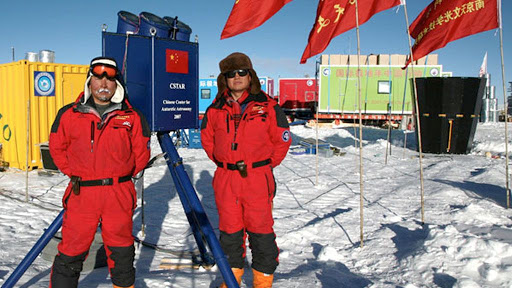
\includegraphics[width=0.6\textwidth]{clo.jpg}
	\caption{穿着防寒服的科考队员}
	\label{clo}
\end{figure}

\subsection{待解决的问题}
问题一:模拟实验者在南极洲长城站外的的工作状态,环境温度为$-40$\textcelsius,无风,工作者的体表温度在15\textcelsius 下时工作很苦难,在10\textcelsius 以下时会有生命危险,建立一个热传递数学模型,分析实验者能在室外坚持多久.

问题二:如果长城站外风速为3m/s,实验者同时做轻微运动,改进问题一建立的模型以模拟实验者面临的环境,计算实验者在滞留在外的最长时间.

问题三:实验者的防寒服最大承受重量为100kg,由于环境影响,每过10s,防寒服的承受重量都会下降,实验者必须要防寒服承受重量下降到自身体重以前进入长城站,如果防护服的材料费用能够增加50\%,如何调整内层,中间层和外层的厚度使得实验尽可能支撑更长时间,防护服各层材料厚度的增加受到费用限制和实际使用能力的限制,另外相应材料厚度的增加需要满足实际情况.

问题四:如果不追加资金,如何通过提升相变材料的放热能力,进而使得实验者能坚持同问题三中一样长的时间,假定放热能力在各个温度下上同比例增加的,请给出具体数值.


\section{模型假设}
\begin{enumerate}
	\item 不考虑衣服各织物层的褶皱及空隙,将织物层视为多层平行材料.
	\item 热量沿垂直于人体核心区皮肤的方向传递,不考虑热量在衣物系统内的纵向扩散.
	\item 在极低温的状态下,不考率热量的辐射传递以及人体的蒸发散热.
	\item 本文考虑的温度范围的极差不大,因此将各温度下的热传导率视为一致的.
	\item 衣服内层空气层的厚度很小,因此不考虑热对流.
\end{enumerate}


\section{符号说明}
\begin{center}
	\begin{tabular}{ccccc}
		\toprule[1.5pt]
		符号 & 含义\\
		\midrule[1pt]
		$k_{0}$ & 热传递系数\\
		$T_{i}$ &服装系统内第i层材料内部温度\\
		$T_{h}$ &人体核心温度\\
		$T_{S}$ &外界温度\\
		$h_{c}$ &对流热交换系数\\
		$A_{b}$ &人体有效表面积\\      
		$W$     &人体所做机械功\\
		$M$     &人体新陈代谢效率\\
		\bottomrule[1.5pt]
		注:表中未说明的符号以首次出现处为准
	\end{tabular}
\end{center}





\section{问题一模型的建立与求解}
\subsection{问题分析}
在实际的低温作业环境下,作业者与环境的热量交换发生在三维环境中,由于不考虑气体沿人体躯干的流动和防护服内热量的横向传播,因此忽略高度与防护服宽度这两个维度,我们可以将问题简化为仅考虑防护服与皮肤厚度这一单一维度上的热传导模型.
\begin{figure}[!htbp]
	\centering
	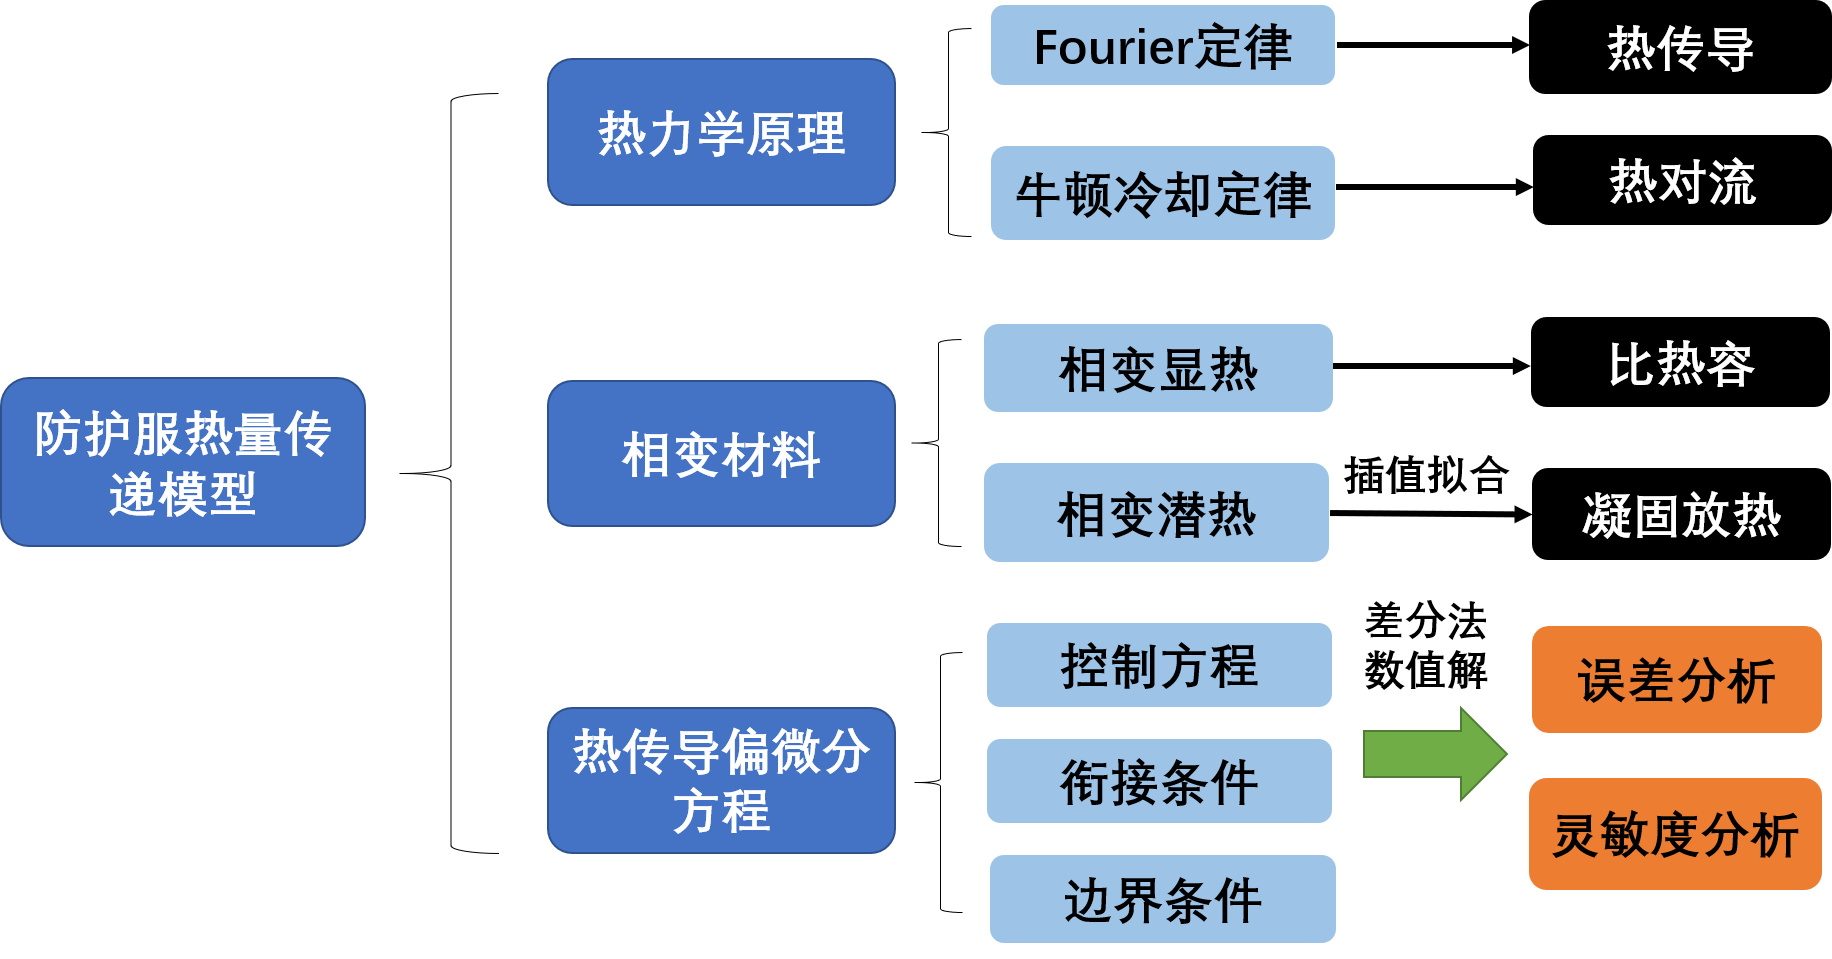
\includegraphics[width=0.6\textwidth]{map1.png}
	\caption{问题一思维导图}
\end{figure} 



\subsection{物理背景}
热量传递主要有三种基本方式:导热,热对流和热辐射.传热过程可能涉及以上一种或多种方式,根据传热介质的特征,热量传递的过程又可以分为热传导,对流传热和辐射传热.由于在超低温下,热量的对外辐射可以忽略不计,所以本文不考虑辐射传热.
\subsubsection{热传导方程}
导热是指依靠物质的分子,原子和电子的振动,位移和相互碰撞而产生热量传递的方式.热传导在气态,液态或者固态的物质中都可以发生,但其热量传递的机理不同,本文在此不做过多解释.

$Fourier$定律是描述热传导现象的基本定律,指出在一维空间内,当物体温度不受外界条件影响时,其热量沿温度降低的方向传递.热传导方程的推倒如下:

假设有一均匀的长细杆,其横截面积为$S_{1}$沿着细杆长度方向有温度变化,其侧面是绝热的,考虑其内部热量传递过程,由于杆是均匀细长的,所以任何时刻都可以将杆的横截面上的温度视为相同的,由于杆侧面是绝热的,所以热量只沿杆长度方向传导,以圆柱的母线为轴,温度由高到低的方向为$x$轴正方向建立以为坐标系.以$u(x,t)$表示杆上坐标为$x$的点在$t$时刻的速度.

设杆的比热容为$c$,$\rho$为杆的密度,我们选择杆上长度为$\Delta x$的一段,研究其在$\Delta t$时间内的温度变化.

在$\Delta t$时间内使得小段温度升高,所需热量为:
\begin{equation}
Q=c\rho S_{1}\Delta x[u(x,t+\Delta t)-u(x,t)].
\end{equation}
由$Foruier$实验定律可知,当一均匀介质内部有温度差时,热量由温度高处向温度低处传递,单位时间内流过单位面积的热量$q$与温度下降率成正比,在一维空间上:
\begin{equation}
q=-k u_{x}.
\end{equation}
其中,$k$为导热系数,在温度相差不是特别大的情况下,可以看做只与材料相关.由$Fourier$定律我们可以求出在$\Delta t$时间内流入或流出短杆的热量.
\begin{equation}
Q_{1}(x)=-ku_{x}(x,t)S_{1}\Delta t,
\end{equation}
\begin{equation}
Q_{2}(x+\Delta x)=-ku_{x}(x+\Delta x,t)S_{1}\Delta t.
\end{equation}
其中$Q_{1}(x)$,$Q_{2}(x+\Delta x)$分别表示流入短杆和流出短杆的热量,根据能量守恒定律:
\begin{equation}
Q=Q_{1}(x)-Q_{2}(x+\Delta x),
\end{equation}
即
\begin{equation}
c\rho u_{t}=\frac{k[u_{x}(x+\Delta x,t)-u_{x}(x,t)}{\Delta x},
\end{equation}
令$\Delta x$趋向于0,两边等式取极限得:
\begin{equation}
u_{t}=\frac{k}{c\rho}u_{xx},
\end{equation}
令$D=\frac{k}{c\rho}$,即有:
\begin{equation}
u_{t}=Du_{xx}.
\end{equation}

\subsubsection{牛顿冷却定律}
防护服与外界热交换的主要方式是热对流,牛顿冷却定律是研究温度高于周围环境的物体向周围媒介传递热量逐渐冷却时所遵循的规律.当物体表面与周围存在温差时,单位时间从单位面积散失的热量与温度差成正比,比例系数称为热传递系数,以$k_{0}$表示.
\begin{equation}
\frac{\partial Q}{\partial t}=k_{0}(T-T_{s}).
\end{equation}

%插入参考文献\upcite{bib:one}.
\subsection{一维非稳态变相材料防寒服热量传递模型的建立}
对于“皮肤-内层空气-防寒服-外部环境”系统,根据热量在相同介质内的传导,在不同介质间的传递,防护服表层与外界环境的对流建立偏微分方程模型.
\begin{figure}[!htbp]
	\centering
	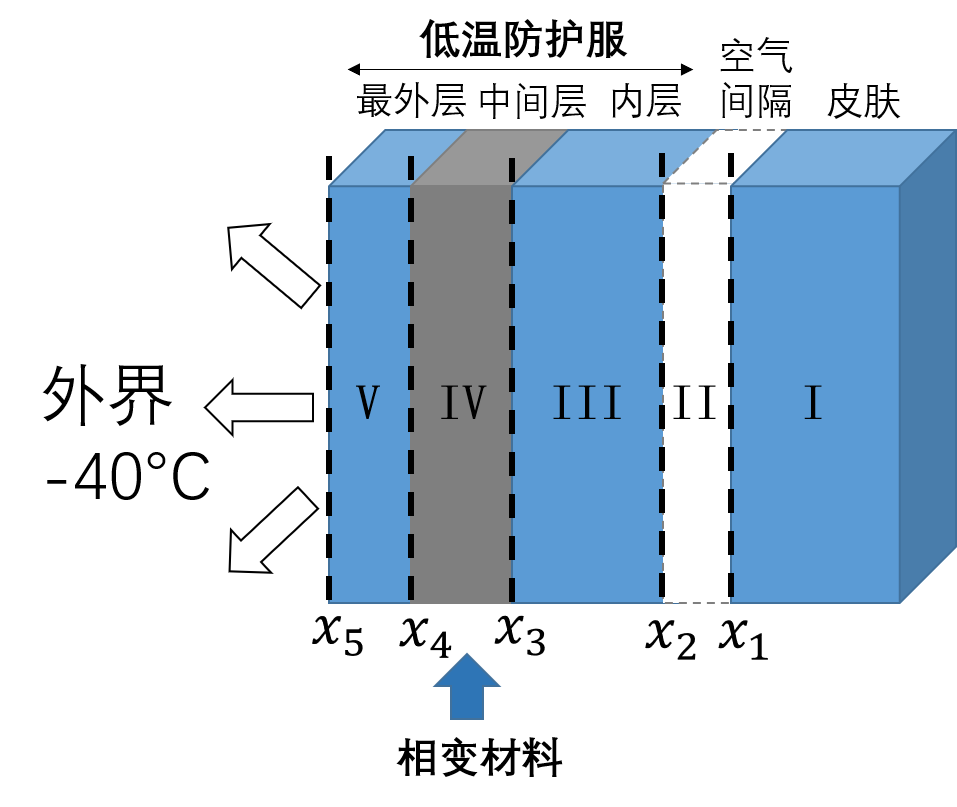
\includegraphics[width=0.6\textwidth]{yanshi.png}
	\caption{防寒服一维简化示意图}
	\label{shiyi}
\end{figure} 

\subsubsection{相同介质内热量传导}
在这里我们探讨的是热量在一般介质中传导的规律,热量在变相材料中的传导将在后面讨论.

\begin{equation}
	\begin{cases} 
	\frac{\partial T_{1}}{\partial t}=D_{1}\frac{\partial^{2}T_{1}}{\partial x^{2}},& 0\leq x \le x_{1},\\
	\frac{\partial T_{2}}{\partial t}=D_{2}\frac{\partial^{2}T_{2}}{\partial x^{2}},& x_{1}\leq x \le x_{2},\\
      \frac{\partial T_{3}}{\partial t}=D_{3}\frac{\partial^{2}T_{3}}{\partial x^{2}},& x_{2}\leq x \le x_{3},\\
      \frac{\partial T_{4}}{\partial t}=D_{4}\frac{\partial^{2}T_{4}}{\partial x^{2}},& x_{3}\leq x \le x_{4},\\
      \frac{\partial T_{5}}{\partial t}=D_{5}\frac{\partial^{2}T_{5}}{\partial x^{2}},& x_{4}\leq x \le x_{5},\\
	\end{cases}
\end{equation}



\subsubsection{初始条件}
我们建立的“皮肤-内层空气-防寒服-外部环境”系统基于一定的初始条件,不妨假设防寒服的各结构的初始温度为30摄氏度,皮肤组织的温度与人体核心温度37摄氏度相同,内层空气的温度为35摄氏度.
\begin{equation}
\begin{cases}
T_{1}(x,0)=T_{h},\\
T_{2}(x,0)=T_{air},\\
T_{3}(x,0)=T_{clo},\\
T_{4}(x,0)=T_{clo},\\
T_{5}(x,0)=T_{clo}.\\
\end{cases}
\end{equation}
其中,$T_{h}=37\textcelsius$代表人体的核心体温,$T_{air}=35\textcelsius$代表初始条件内层空气温度,$T_{clo}=30\textcelsius$代表衣物的初始温度.

\subsubsection{不同介质衔接处热量传递}
假设各介质层是平整无缝隙相连的,即两种介质之间没有空气或其他介质,近似看成无缝对接.在系统内4处衔接点的状态方程为:
\begin{equation}
\begin{cases} 
T_{1}(x_{1}-0,t)=T_{2}(x_{1}+0,t),\\
k_{1} \frac{\partial T_{1}}{\partial x}\big|_{x=x_{1}-0}=k_{2} \frac{\partial T_{2}}{\partial x}\big|_{x=x_{1}+0}.\\
T_{2}(x_{2}-0,t)=T_{3}(x_{2}+0,t),\\
k_{2} \frac{\partial T_{2}}{\partial x}\big|_{x=x_{2}-0}=k_{3} \frac{\partial T_{3}}{\partial x}\big|_{x=x_{2}+0}.\\
T_{3}(x_{3}-0,t)=T_{4}(x_{3}+0,t),\\
k_{3} \frac{\partial T_{3}}{\partial x}\big|_{x=x_{3}-0}=k_{4} \frac{\partial T_{4}}{\partial x}\big|_{x=x_{3}+0}.\\
T_{4}(x_{4}-0,t)=T_{5}(x_{4}+0,t),\\
k_{4} \frac{\partial T_{4}}{\partial x}\big|_{x=x_{4}-0}=k_{5} \frac{\partial T_{5}}{\partial x}\big|_{x=x_{4}+0}.\\
\end{cases}
\end{equation}
\subsubsection{边界条件}
人体内层皮肤的温度与人体核心相当,可以给出$Dirichlrt$右边界边值条件.
\begin{equation}
T_{1}(0,t)=T_{h},
\end{equation}
同时外层隔热层与外界进行热对流,根据牛顿冷却定律,给出$Robin$左边界条件:
\begin{equation}
\frac{\partial T_{5}}{\partial{t}}\big|_{x=x_{5}}=h_{c}\times[T_{5}(x_{5},t)-T_{s}].
\end{equation}
其中$h_{c}$为对流热交换系数,$h_{c}$的公式如下:
\begin{equation}
h_{c}=2.38(T_{5}(x_{5},t)-T_{s})^{0.25}.
\end{equation}
对流热交换系数在外界与衣服表面温度差异不大时,差距不大,可以看做以常数.

\subsubsection{热量在变相材料中的传递}
当变相材料的温度下降到一定阈值时,其会通过形态变化放热以延缓热量流出的速率.
一段变相材料上的热传导过程除满足方程(2)(3)(4)外,其释放的能量也可以看做是在$\Delta t$时间内流入短杆的热量.
\begin{equation}
Q_{3}= m_{\Delta x}\times DSC \times \Delta t,
\end{equation}
$m_{\Delta t}$表示这小段变相材料的质量.
\begin{equation}
m_{\Delta t}=S_{1}\Delta x\times \rho,
\end{equation}
根据能量守恒定律:
\begin{equation}
Q=Q_{1}+Q{3}-Q{2},
\end{equation}
化简,两边除以$c\rho S_{1}\Delta x\Delta t$,
\begin{equation}
\frac{\partial T_{4}}{\partial t}==D_{4}\frac{\partial^{2}T_{4}}{\partial x^{2}}-\frac{DSC}{c}.
\end{equation}

\subsubsection{模型综述}
\begin{equation}
\begin{cases}
\text{控制方程:}&\begin{cases}\frac{\partial T_{i}}{\partial t}=D_{i}\frac{\partial^{2}T_{i}}{\partial x^{2}},x_{i-1}\leq x \le x_{i},i=1,2,3,5.\\
\frac{\partial T_{4}}{\partial t}==D_{4}\frac{\partial^{2}T_{4}}{\partial x^{2}}-\frac{DSC}{c},\text{$DSC$是关于$T_{4}$的一个函数}.\\
\end{cases}.\\
\text{接触面:}&\begin{cases}T_{i}(x_{i}-0,t)=T_{i+1}(x_{i}+0,t),i=1,2,3,4.\\
k_{i} \frac{\partial T_{i}}{\partial x}\big|_{x=x_{i}-0}=k_{i+1} \frac{\partial T_{i+1}}{\partial x}\big|_{x=x_{i}+0},i=1,2,3,4\\
\end{cases}\\
\text{边界条件}&\begin{cases}T_{5}(x_{5},t)=T_{s},\\
\frac{\partial T_{5}}{\partial{t}}\big|_{x=x_{5}}=h_{c}\times[T_{5}(x_{5},t)-T_{s}].\\
\end{cases}\\
\text{初始条件;}& T_{i}(x,0)=T_{i},T_{i}\text{表示各介质初始温度}\\
\end{cases}
\end{equation}

\subsection{模型求解}
\subsubsection{人体相关参数求解}
服装系统通过热对流向外界传递热量,其对流热量公式如下:
\begin{equation}
\Delta C=h_{c}A_{b}(T_{5}(x_{5},t)-T_{s}).
\end{equation}
其中,$T_{5}(x_{5},t)$为服装表面温度,$T_{s}$为外部环境温度,$A_{b}$为人体有效表面积.

\textbf{人体体表面积:}人体表面积可以用$Stevenson$的金典面积公式计算出人体体表面积,其公式如下:
\begin{equation}
S=0.61\times h+0.0128\times w-0.1529.
\end{equation}
其中,$h$为人体身高,$w$为人体体重.

\textbf{有效体表面积:}
相变防护服是背心结构款式,只能对身体的核心部位,胸部,背部,腹部和臀部进行保护,因此需要取腹部和臀部有效面积的一半,根据$ISO9920$\upcite{bib:four}人体划分标准,我们得到的人体有效表面积百分比系数为:
\begin{equation}
N=10.2\%+9.2\%+\frac{6.1\%}{2}+\frac{6.6\%}{2}=25.75\%.
\end{equation}
求出来的人体体表面积$S$为1.6521平方米,有效体表面$S_{A}$为0.425平方米.

\subsubsection{相变材料放热能力三次样条插值}
附件一种给出了在不同温度下相变材料的放热数据,我们是用三次样条插值进行拟合,该方法通过求解三弯矩方程组得出曲线函数,划分$\Delta: a<T_0<T_1<...<T_n=b$,添加3(n-1)个光滑约束.最后两者的拟合误差为$2.0226\times 10^{-5}$

\begin{equation}
\left\{
\begin{array}{l}
	S(x_i-0)=S(x_i+0) \\
S'(x_i-0)=S'(x_i+0) \\
S''(x_i-0)=S''(x_i+0) 
\end{array} \right.
\end{equation}
\begin{figure}[!htbp]
	\centering
	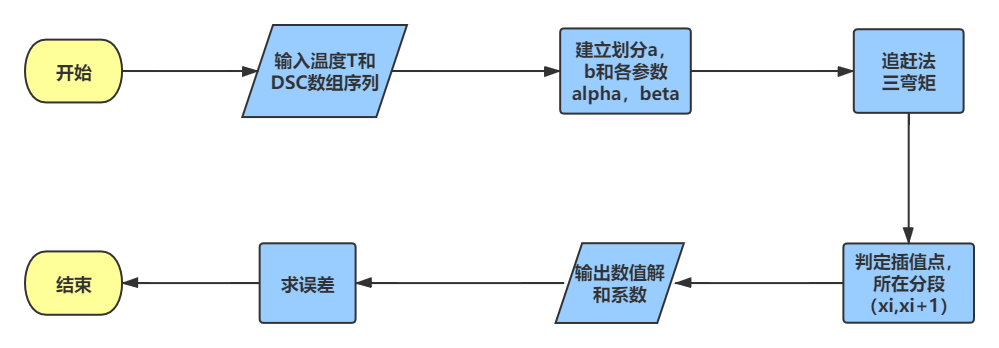
\includegraphics[width=0.8\textwidth]{3ci2.png}
	\caption{三次样条插值流程图}
\end{figure}

\begin{figure}[!htbp]
	\centering
	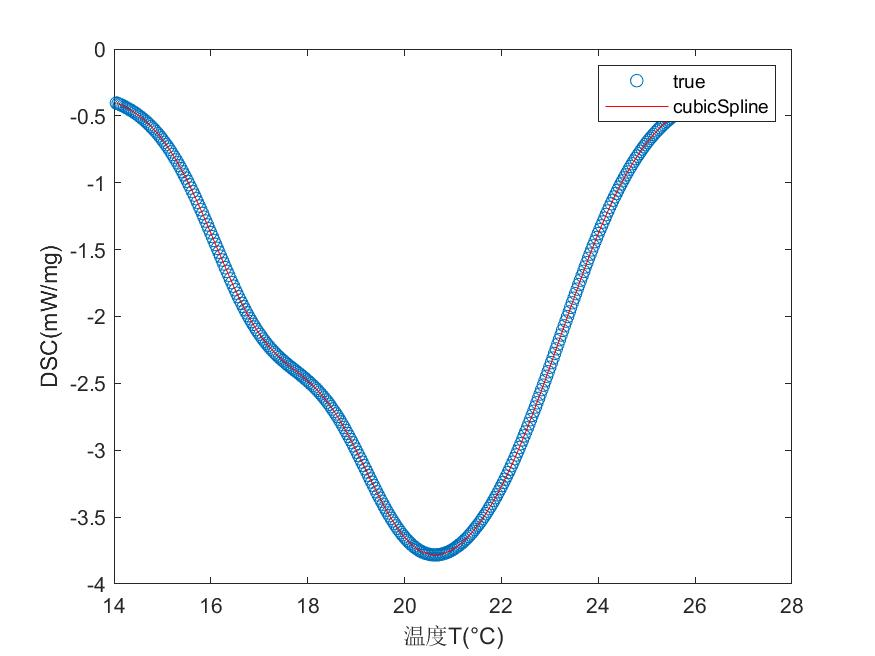
\includegraphics[width=0.6\textwidth]{out.jpg}
	\caption{相变材料三次样条拟合}
\end{figure}

\subsubsection{热传导方程有限差分法}
对于本文设计到的微分方程组求解问题,常常难以找到微分方程的解析解,因此因当求出其数值解,求解偏微分方程的方法有有限元法和有限差分法.

本文采用有限差分法处理微分方程组,借助$Taylor$展开公式,将约束方程中的导数用网络节点的函数值的插上代替来进行离散,建立以网格上点的值为未知数的代数方程组.其基本思想是将连续定界区域用有限个离散点构成的网格代替,离散点成为网络节点;将连续定界区域内连续变量的函数用在网格上定义的离散遍变量函数近似,用房层和定界条件中的微商用插上近似,积分用积分和来近似,于是原微分方程组和定解条件就近似地替代为代数方程组,即有限差分方程组,解此方程组可以得到原问题在离散点上的近似解,然后再利用插值法便可以从离散解得到定解问题在整个区域上的近似解.

$Crank-Nicolson$方法是有限差分法中一种,其余方法包括古典显方法和古典隐方法.它是一种在时间方向上隐式的二阶方法,该办法诞生于20世纪,由$John Crank$和$Phyllis Nicolson$发展,$Crank Nicolson$方法被证明是无条件稳定的,但是如果时间步长与空间步长平方的比值过大,近似解中将会存在虚假的震荡或衰减.本题建立的模型影响因素较多,时间较长,因此我们选择了精准度较差的后向欧拉方法进行计算.

$Crank-Nicolson$方法在空间域上进行中心差分,时间阈上应用剃度公式,保证了时间域上的二阶收敛.令$T(i\Delta x,n\Delta t)=T_{i}^{n}$.
\begin{equation}
\frac{u_{i}^{n+1}-u_{i}^{n}}{\Delta t}=F_{i}^{n}\big(u,x,t,\frac{\partial u}{\partial x},\frac{\partial^{2}u}{\partial x^2}),
\end{equation}
\begin{equation}
\frac{u_{i}^{n+1}-u_{i}^{n}}{\Delta t}=F_{i}^{n+1}\big(u,x,t,\frac{\partial u}{\partial x},\frac{\partial^{2}u}{\partial x^2}),
\end{equation}
\begin{equation}
\frac{u_{i}^{n+1}-u_{i}^{n}}{\Delta t}=\frac{1}{2}\big(=F_{i}^{n+1}\big(u,x,t,\frac{\partial u}{\partial x},\frac{\partial^{2}u}{\partial x^2})+F_{i}^{n}\big(u,x,t,\frac{\partial u}{\partial x},\frac{\partial^{2}u}{\partial x^2})).
\end{equation}


\textbf{中心差分:}
\begin{equation}
\frac{T_{i}^{n+1}-T-{i}^n}{\Delta t}=\frac{1}{2}[(D_{i}^{n+1}\frac{\partial^{2}T}{\partial x^{2}})+(D_{i}^{n}\frac{\partial^{2}T}{\partial x^{2}})].
\end{equation}

我们首先对于该问题构建出了二维平面,该网格分别取$\Delta x$和$\Delta t$方向为步长,用两组平行之间对时间,空间构成的网格进行构造然后利用其平行直线来划分网格,从而得到$T(x,t)$,并对网格内的点的$\frac{\partial T}{\partial t}$,$\frac{\partial^2 T}{\partial x^2}$采用欧拉法,得到热传导差分方程.最终得到他介质内的迭代过程.
\begin{figure}[!h]
	\centering
	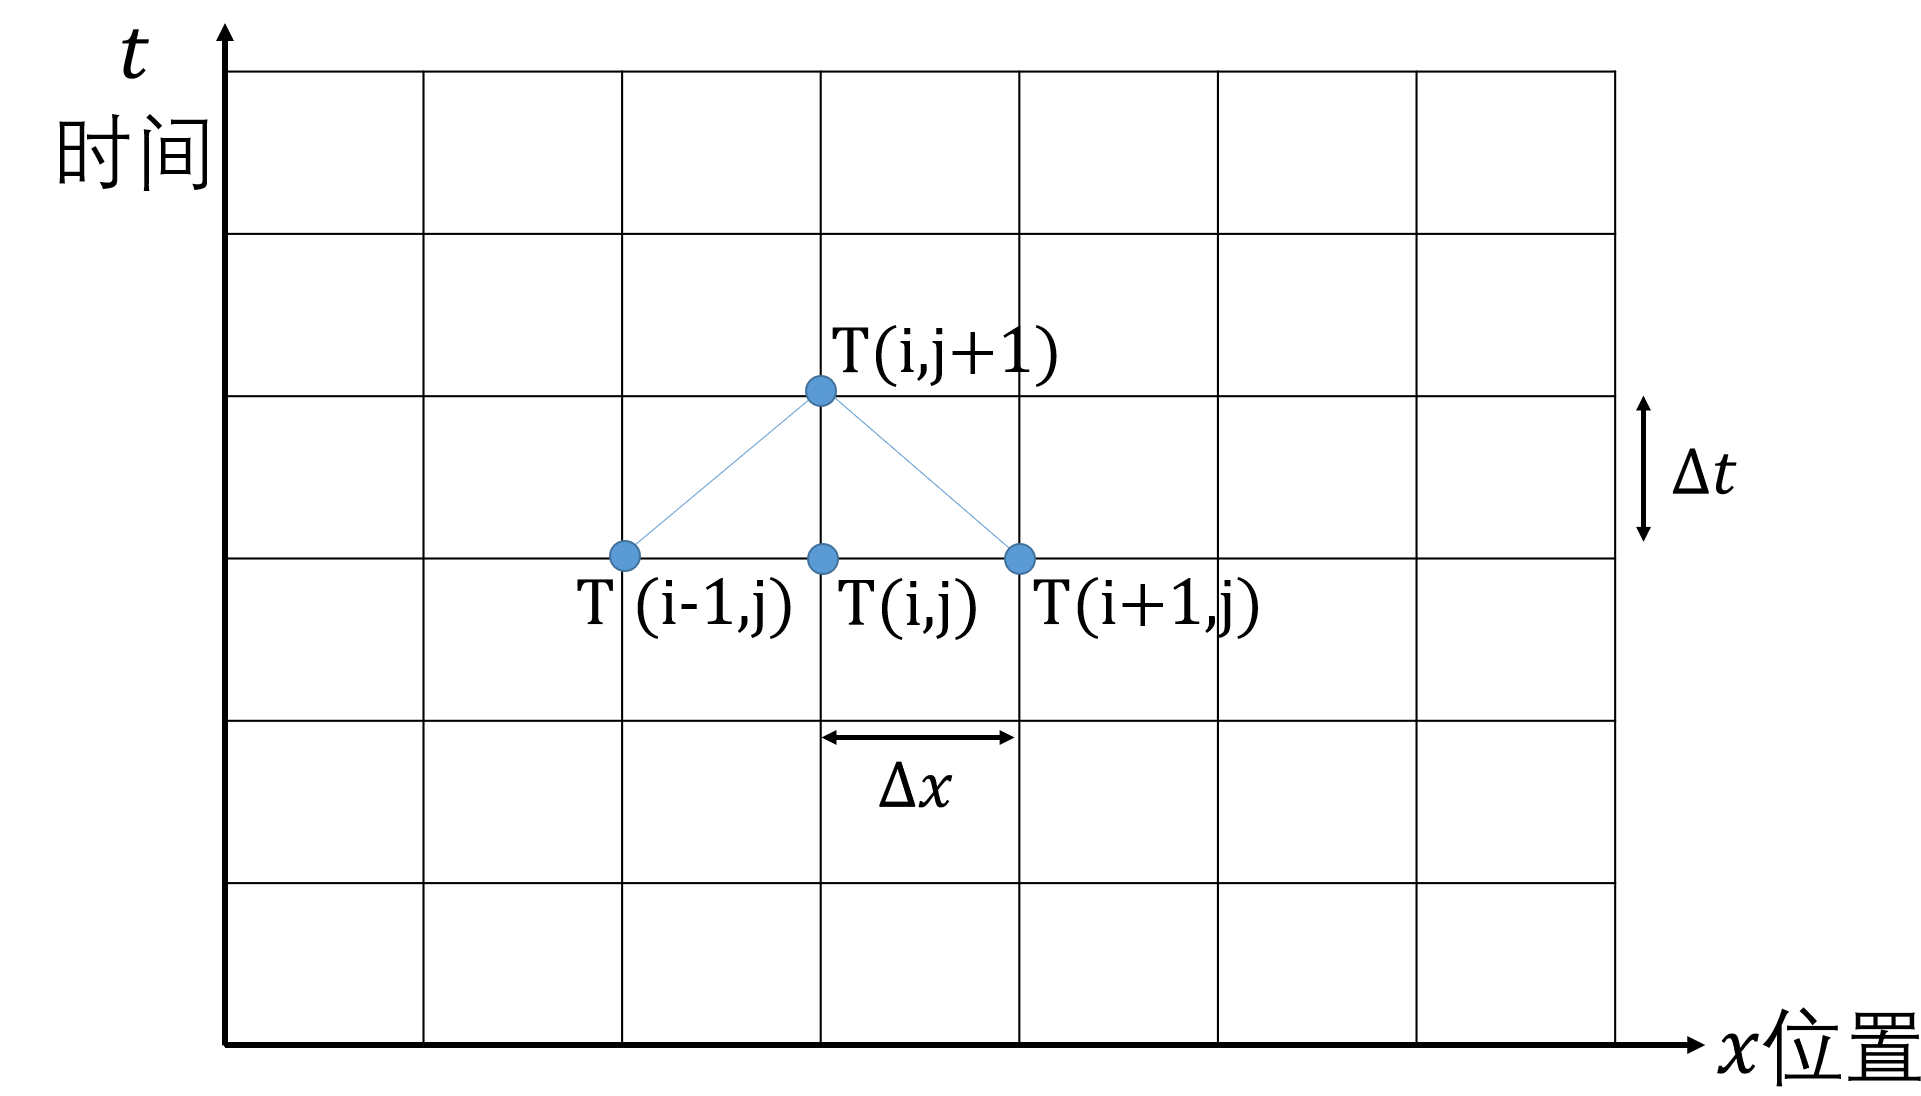
\includegraphics[width=0.8\textwidth]{chafenshiyi.png}
	\caption{差分计算示意图}	
\end{figure}
\begin{equation}
\frac{T(i,j+1)-T(i,j)}{\Delta t}=D\frac{T(i+1,j)-2T(k,j)+T(i-1,j)}{(\Delta x)^2}.
\end{equation}
从而得到热传导的\textbf{控制方程}为
\begin{equation}
	\Delta x_j \rho_j c_j \frac{T_i^{n+1}-T_i^{n}}{\Delta t}=\lambda_j \frac{T_{i+1}^n-2T_i^n+T_{i-1}^n}{\Delta x_j}.
\end{equation}

\textbf{接触面:}

在得到上述控制方程之后我们需要进一步考虑接触面位置的差分迭代公式,有上述的式12我们可以得出的是
\begin{equation}
\lambda_i \frac{T_i-T_(i-1)}{\Delta t}=\lambda_{i+1} \frac{T_{i+1}-T_{i}}{\Delta t}.
\end{equation}
利用中心差分的方法可以得出

\begin{equation}
\frac{1}{2}\left(\Delta x_{j} \rho_{j} c_{j}+\Delta x_{j+1} \rho_{j+1} c_{j+1}\right) \frac{T_{i}^{n+1}-T_{i}^{n}}{\Delta t}=\lambda_{j} \frac{T_{i-1}^{n}-T_{i}^{n}}{\Delta x_{j}}+\lambda_{j+1} \frac{T_{i+1}^{n}-T_{i}^{n}}{\Delta x_{j+1}}.
\end{equation}

\textbf{相变材料部分:}

而在相变材料的时候我们需要考虑DSC的部分和操作,并利用我们在之前所写的公式
\begin{equation}
\frac{\partial T_{4}}{\partial t}=D_{4} \frac{\partial^{2} T_{4}}{\partial x^{2}}-\frac{D S C}{c}.
\end{equation}
从而会得到
\begin{equation}
\Delta x_j \rho_j c_j \frac{T_i^{n+1}-T_j^{n}}{\Delta t}=\lambda_j \frac{T_{i+1}^n-2T_i^n+T_{i-1}^n}{\Delta x_j}-\frac{DSC(T_4)}{c}.
\end{equation}

\textbf{热对流部分:}

对于在对流处的问题我们则需要利用第三类边界条件来建立等式,即就是傅里叶热传导方程的热流密度与牛顿冷却公式比如说我们在第一次通过使用牛顿冷却公式来完成操作,从而从等式的角度建立起差分方程.
\begin{equation}
-\left.\lambda_{1} \frac{\partial T}{\partial x}\right|_{x=0}=h_{c}\left(T_{s}-T(0, t)\right).
\end{equation}

\begin{equation}
\frac{1}{2} \Delta x_{i} \rho_{i} c_{i} \frac{T_{i}^{n+1}-T_{i}^{n}}{\Delta t}=-h_{1}\left(T_{1}^{n}-T_{s}\right)-\lambda_{1} \frac{T_{i}^{n}-T_{i}^{n}}{\Delta x_{i}}.
\end{equation}

%\begin{equation}
%M_{i}=\frac1{WH}\sum_{i=0}^{H-1}\sum_{j=0}^{W-1}I(i,j)
%\end{equation}
%\begin{equation}
%V_{i}=\frac1{WH}\sum_{i=0}^{H-1}\sum_{j=0}^{W-1}({I(i,j)-M_{i})^2}
%\end{equation}

%
%\begin{equation}
%\begin{figure}[!h]
%	\centering
%	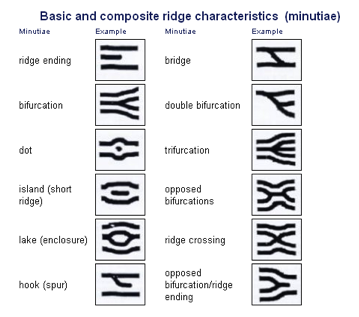
\includegraphics[width=0.8\textwidth]{class.png}
%	\caption{细节点类型示意图}
%	
%\end
%$$ $$
%\end{equation}




%\begin{tabular}{|c|c|c|c|c|c|c|c|c|c|r|}
%	\hline
%	$\delta$$x_{1}$ & $\delta$$ y_{1}$ & $t_{1}$ & $k_{1}$ & $\delta$$ x_{2}$ & $\delta $$y_{2}$ & $t_{2}$ & $k_{2}$ & ... & $t_{20}$ & $k_{20}$\\
%	\hline
%\end{tabular}
\subsection{结果分析}
实验者站在南极洲长城站附近,当时环境安静,晴天无风,-40\textcelsius 在该问题中,由于人体没有运动,我们可认为该人体的新陈代谢保持正常水平,核心体温为37 \textcelsius ,通过热传导和热对流两类热量传递方程,通过综合计算最终得到了该人在南极寒温下\textbf{工作571.86s}后人体皮肤会下降到\textbf{15} \textcelsius 以下\textbf{难以再进行工作},\textbf{1539.70s}后会降低到\textbf{10} \textcelsius 以下会有\textbf{生命危险}.图\ref{fig:T_surface_prob1}中我们模拟了该人体在该环境中的降温状况.
\begin{figure}[!htbp]
	\centering
	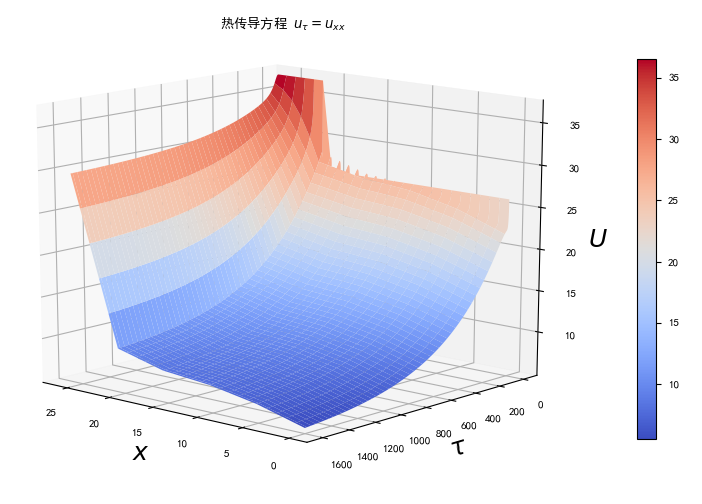
\includegraphics[width=0.6\textwidth]{T_surface_prob1.png}
	\caption{人体—防护服—外界整体降温模拟过程}
	\label{fig:T_surface_prob1}
\end{figure} 

\begin{figure}[!h]
\begin{minipage}[t]{0.48\textwidth}
	\centering
	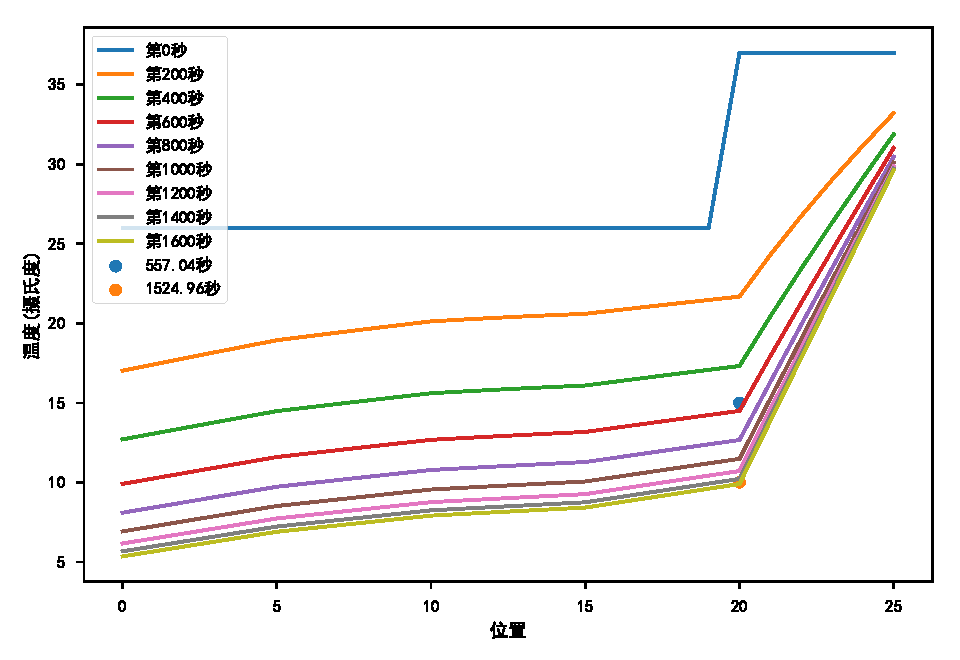
\includegraphics[width=0.95\textwidth]{T_sliceprob1.pdf}
	\caption{人体—防护服—外界系统各位置不同时刻的温度变化曲线}
\end{minipage}
\begin{minipage}[t]{0.48\textwidth}
	\centering
	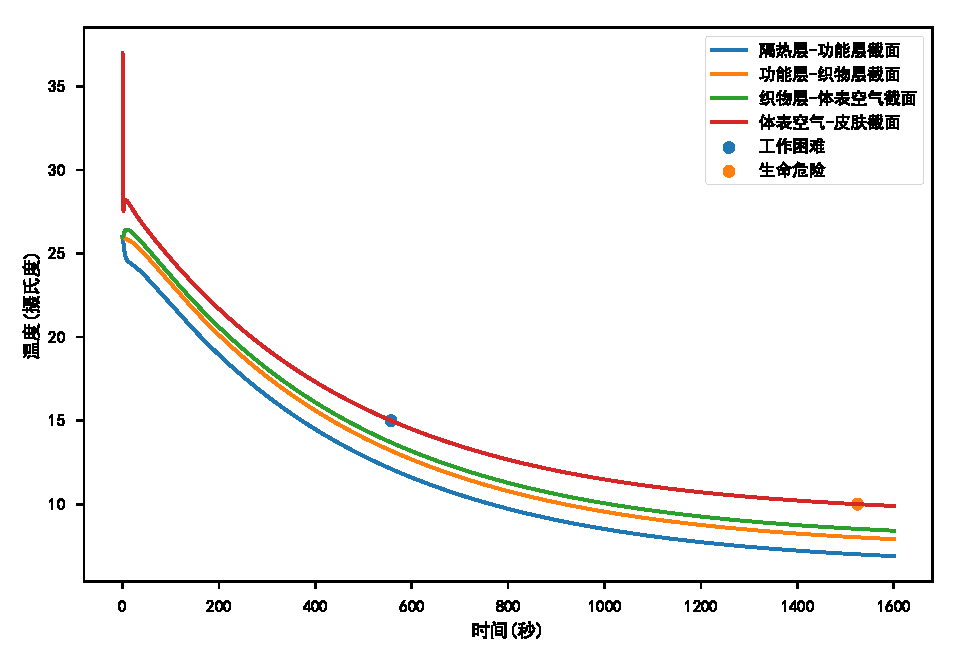
\includegraphics[width=0.95\textwidth]{x_sliceprob1.pdf}
\caption{各接触面不同时刻的温度变化曲线}
\end{minipage}
\end{figure}

%\begin{figure}[!htbp]
%	\centering
%	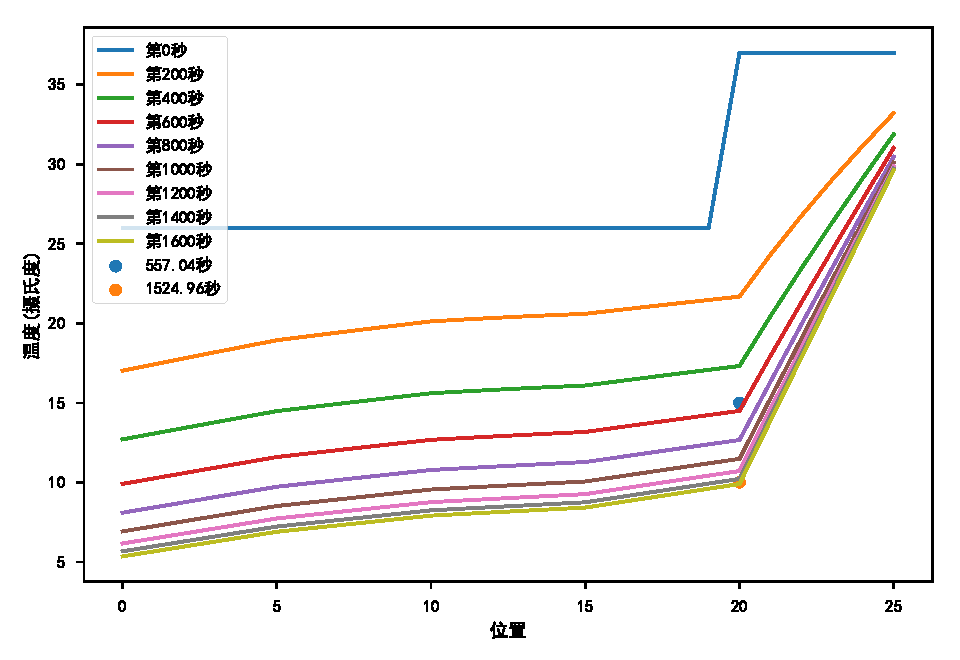
\includegraphics[width=0.6\textwidth]{T_sliceprob1.pdf}
%	\caption{人体—防护服—外界系统各位置不同时刻的温度变化曲线}
%\end{figure} 
%\begin{figure}[!htbp]
%	\centering
%	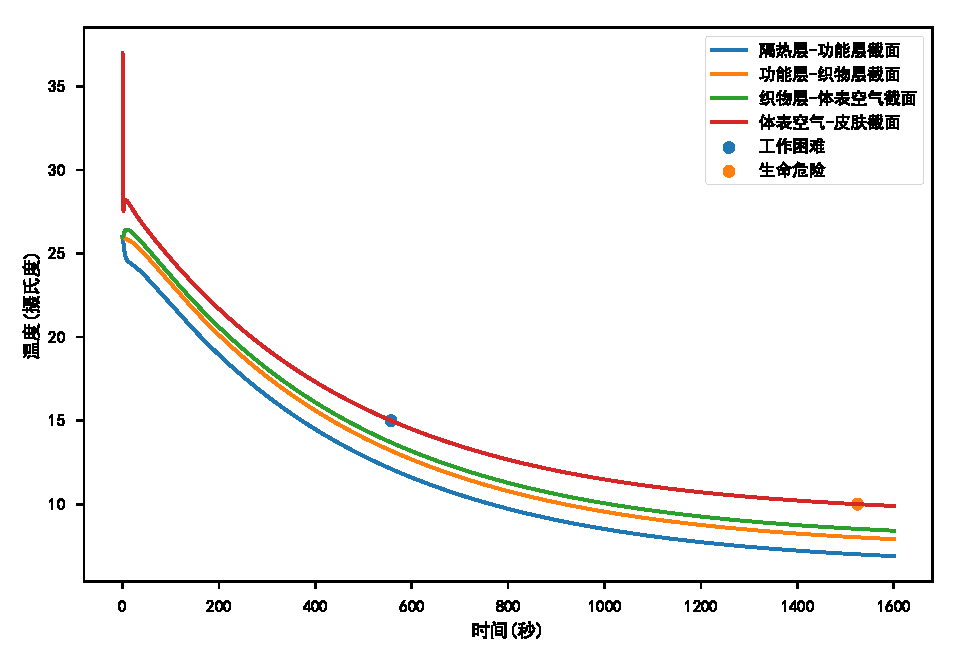
\includegraphics[width=0.6\textwidth]{x_sliceprob1.pdf}
%	\caption{各接触面不同时刻的温度变化曲线}
%\end{figure} 

\subsection{灵敏度分析}
我们通过改变空气层和皮肤层的厚度来衡量该模型对于人体皮肤降温过程的影响,从图\ref{fig:th_air_sensitivity}和图\ref{fig:th_skin_sensitivity}中,可以看出来在合理的范围内,人体皮肤与服装最内层的空气间隔增大和皮肤厚度增大对于降温速率的影响较小,说明\textbf{模型具有稳定性.}
\begin{figure}[!h]
	\begin{minipage}[t]{0.48\textwidth}
		\centering
	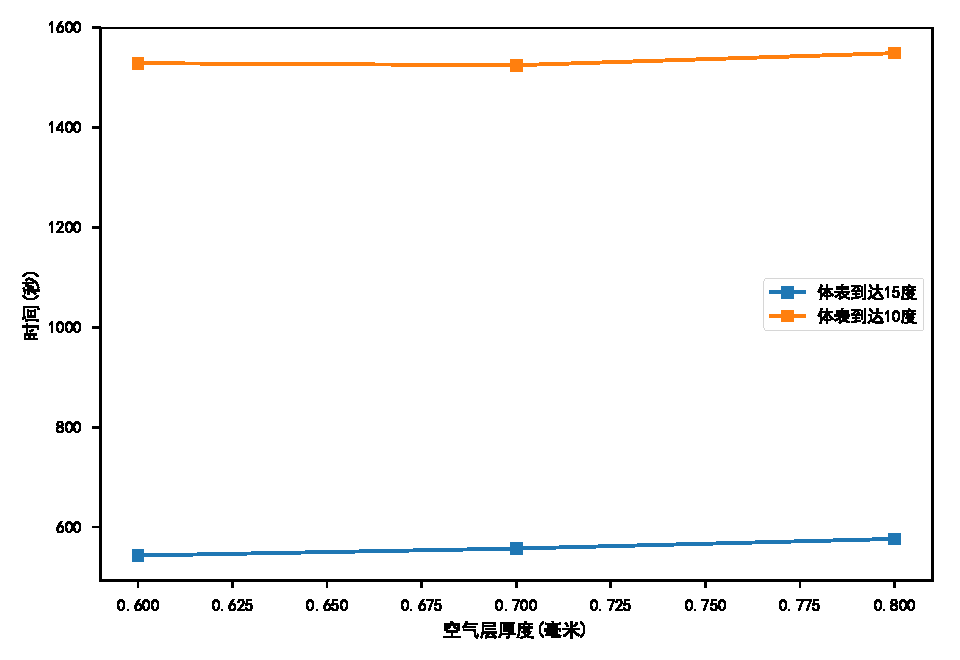
\includegraphics[width=0.95\textwidth]{th_air_sensitivity.pdf}
		\caption{空气层厚度对降温速率的影响}
		\label{fig:th_air_sensitivity}
	\end{minipage}
	\begin{minipage}[t]{0.48\textwidth}
		\centering
	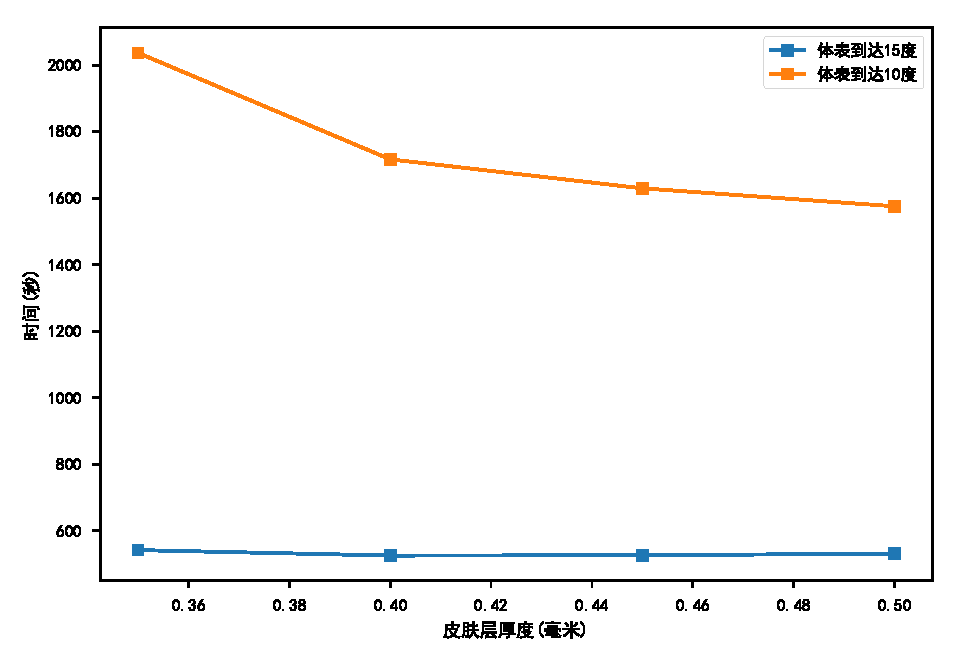
\includegraphics[width=0.95\textwidth]{th_skin_sensitivity.pdf}
\caption{皮肤厚度对降温速率的影响}
\label{fig:th_skin_sensitivity}
	\end{minipage}
\end{figure}
%\begin{figure}[!htbp]
%	\centering
%	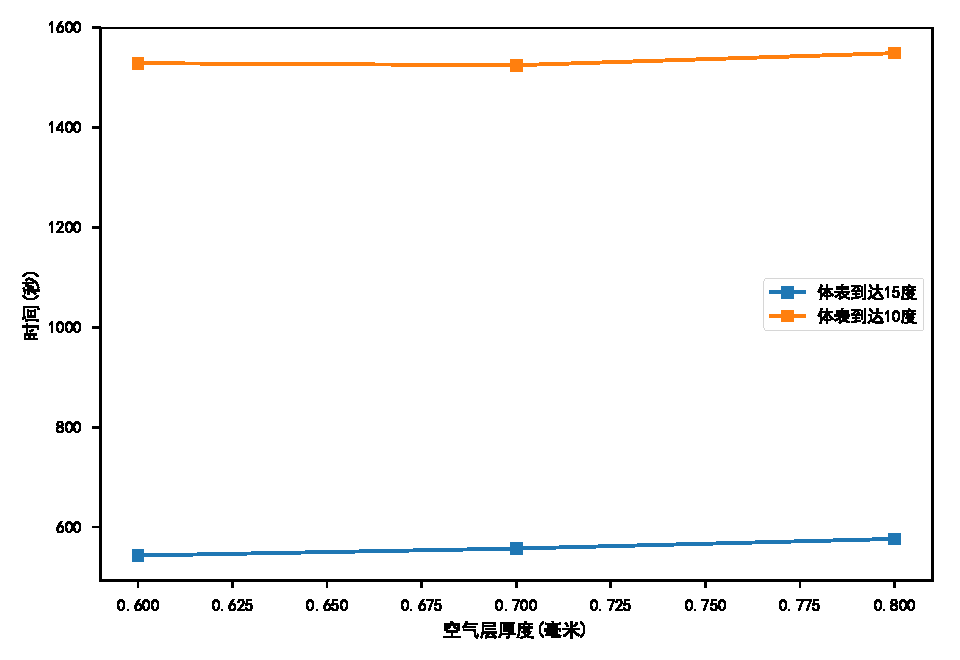
\includegraphics[width=0.6\textwidth]{th_air_sensitivity.pdf}
%	\caption{空气层厚度对降温速率的影响}
%\end{figure} 
%
%\begin{figure}[!htbp]
%	\centering
%	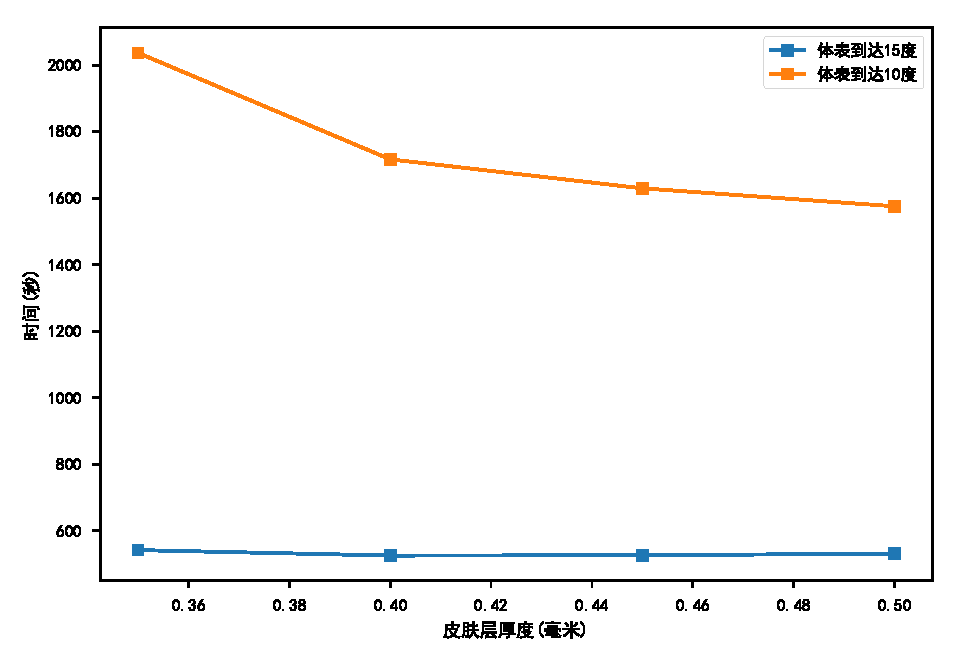
\includegraphics[width=0.6\textwidth]{th_skin_sensitivity.pdf}
%	\caption{皮肤厚度对降温速率的影响}
%\end{figure} 

\section{问题二模型的建立与求解}
\subsection{低温环境下的人体热平衡分析}
人体通过产热和散热机制来稳定正常的体温,新陈代谢以维持人体各器官的生理活动及及时步长由于各种情况造成的热量损失,不同环境温度对人体新陈代谢有显著的影响.人体的核心温度保持在37\textcelsius 左右,人体向周围环境的防热属于物理性体温调教,通过传导,对流,辐射和增发四种方式进行,在极低温条件下,不考虑辐射和蒸发这两种方式,如果服装的保热能力不够,那么通过服装表面的对流散热将会显著的超过人体代谢的产热量,同时人体通过呼吸散失的热量也会增加,这些超出产热量的散热会使人体正常热平衡遭到破坏.

人体新陈代谢产生的热量一部分转化为外部机械功,一部分转化为体内热量,但是做功的机械效率是很小的,常保持在0-20\%,而且绝大多数活动的机械效率为0,对于低温环境精致或轻微活动的人,其做功为0,人体单位面积产热为单位面积新陈代谢率.

\begin{figure}[!htbp]
	\centering
	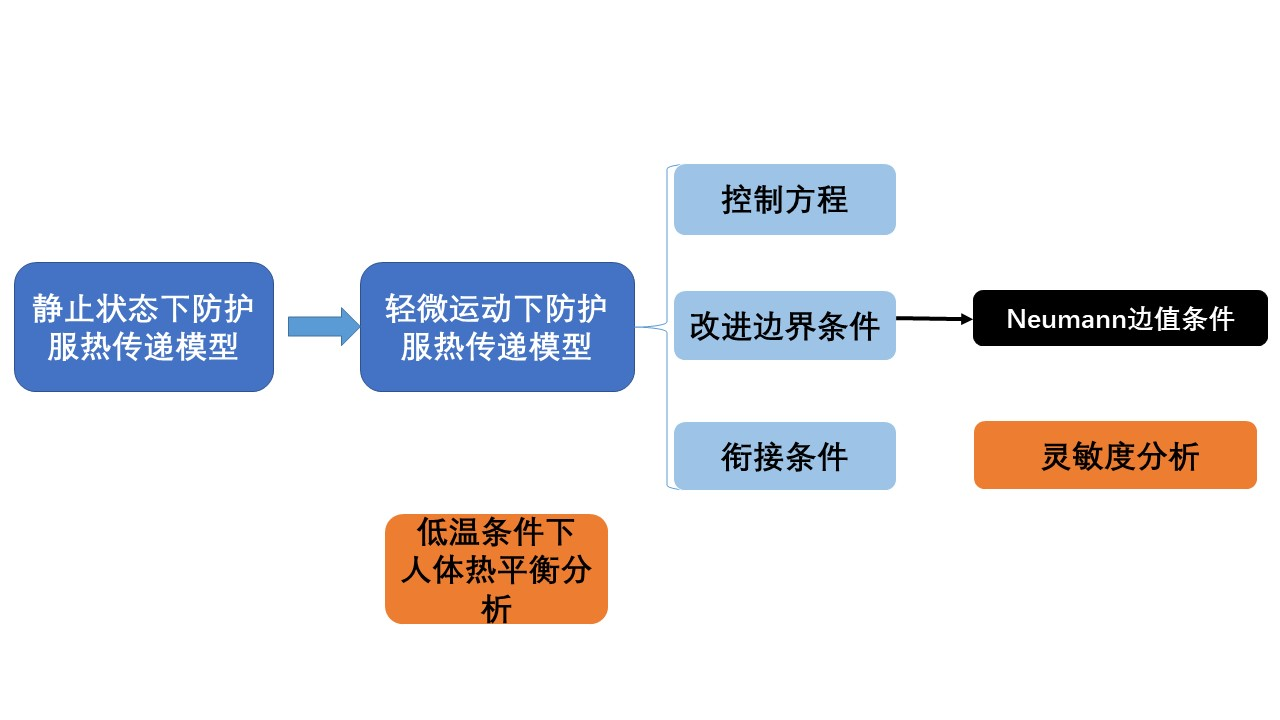
\includegraphics[width=0.8\textwidth]{mindmap2.jpg}
	\caption{问题二思维导图}
\end{figure}

\subsection{人体产热防寒服温度传导模型的建立}
\subsubsection{人体产热量}
低温环境中人体单位时间的产热量$\Delta H$为:
\begin{equation}
\Delta H=(M-W)\times S\times N,
\end{equation}
其中$M$为人体新陈代谢率,$W$表示外部机械功.

人体所做机械功为:
\begin{equation}
W=\mu M.
\end{equation}
$\mu$为做功占新陈代谢的比例,一般去5\%左右,由于机械效率基本为0,所以低温环境中单位时间的产热量为:
\begin{equation}
\Delta H=M\times S.
\end{equation}
通过查找相应参考文献\upcite{bib:four},我们获得了人体在静止或者轻微运动状态时的\textbf{代谢产热率为$70W/m^{2}$.}



\subsubsection{新陈代谢下皮肤内侧边界的热传导方程}
我们对问题一建立的模型进行改进,模型一中我们认为人的皮肤内表层保持恒温,绝对值等于人体核心温度37\textcelsius ,但由于处在极冷环境中,人体除核心区域之外的部分温度难以保持恒定,但是在低温环境中,人体向外释放热量以维持体温的能力使可以估计的,我们以其代谢产热率替代\upcite{bib:two},为此改进模型一的边界条件:将人体代谢率视为系统中端点处的热流密度$q_0$,给出$Neumann$右边界初值条件.

\begin{equation}
q_0=-k_{1}\frac{\partial T_{1}}{\partial x}\big|_{x=0}.
\end{equation}

\subsubsection{模型综述}
将上述对于皮肤内测层的热传导和风速影响的最外侧的对流层系数变化在第一问的模型基础上进行改进,从而得到了新条件下的低温变相材料防寒服热量传递模型.

\begin{equation}
\begin{cases}
\text{控制方程:}&\begin{cases}\frac{\partial T_{i}}{\partial t}=D_{i}\frac{\partial^{2}T_{i}}{\partial x^{2}},x_{i-1}\leq x \le x_{i},i=1,2,3,5.\\
\frac{\partial T_{4}}{\partial t}==D_{4}\frac{\partial^{2}T_{4}}{\partial x^{2}}-\frac{DSC}{c},\text{$DSC$是关于$T_{4}$的一个函数}.\\
\end{cases}.\\
\text{接触面:}&\begin{cases}T_{i}(x_{i}-0,t)=T_{i+1}(x_{i}+0,t),i=1,2,3,4.\\
k_{i} \frac{\partial T_{i}}{\partial x}\big|_{x=x_{i}-0}=k_{i+1} \frac{\partial T_{i+1}}{\partial x}\big|_{x=x_{i}+0},i=1,2,3,4\\
\end{cases}\\
\text{皮肤内测新陈代谢导热}&q_0=-k_{1}\frac{\partial T_{1}}{\partial x}\big|_{x=0}.\\
\text{对流面边界条件}&\frac{\partial T_{5}}{\partial{t}}\big|_{x=x_{5}}=h_{c}\times[T_{5}(x_{5},t)-T_{s}].\\

\text{初始条件}& T_{i}(x,0)=T_{i},T_{i}\text{表示各介质初始温度}\\
\end{cases}
\end{equation}

\subsection{模型求解}
相比于问题一而言该问题只是在模型一的基础上增加了人体的机械能运动产热还有外界风速的变化,那么对于模型一而言,我们改变的部分主要是皮肤层的热量传导,和最外层的对流散热情况,所以在控制方程和边界条件出我们需要在第一问的基础上对皮肤内部热流密度$q_0$和热对流系数$h_c$修改,并利用有限差分法的格式进行迭代分析.
\begin{equation}
\begin{cases}
\text{控制方程:}&
	\Delta x_j \rho_j c_j \frac{T_i^{n+1}-T_i^{n}}{\Delta t}=\lambda_j \frac{T_{i+1}^n-2T_i^n+T_{i-1}^n}{\Delta x_j}\\

\text{接触面:}& \lambda_i \frac{T_i-T_(i-1)}{\Delta t}=\lambda_{i+1} \frac{T_{i+1}-T_{i}}{\Delta t}\\

\text{相变材料层:}& \Delta x_j \rho_j c_j \frac{T_i^{n+1}-T_j^{n}}{\Delta t}=\lambda_j \frac{T_{i+1}^n-2T_i^n+T_{i-1}^n}{\Delta x_j}-\frac{DSC(T_4)}{c}\\

\text{边界条件}&\frac{1}{2} \Delta x_{i} \rho_{i} c_{i} \frac{T_{i}^{n+1}-T_{i}^{n}}{\Delta t}=-h_{c}\left(T_{1}^{n}-T_{s}\right)-\lambda_{1} \frac{T_{i}^{n}-T_{i}^{n}}{\Delta x_{i}}\\

\text{皮肤内侧:}&q_0=-k_{1}\frac{T_1^{n+1}-T_1^n}{\Delta t}\\
\end{cases}
\end{equation}
%\begin{equation}
%\left\{\begin{array}{l}
%\frac{1}{2} \Delta x_{1} \rho_{1} c_{1} \frac{T_{1}^{n+1}-T_{1}^{n}}{\Delta t}=-h_{1}\left(T_{1}^{n}-T_{e n}\right)-\lambda_{1} \frac{T_{1}^{n}-T_{2}^{n}}{\Delta x_{1}} \\
%\frac{1}{2} \Delta x_{4} \rho_{4} c_{4} \frac{T_{e n d}^{n+1}-T_{e n d}}{\Delta t}=-h_{2}\left(T_{e n d}^{n}-T_{s k i n}\right)+\lambda_{4} \frac{T_{e n d-1}^{n}-T_{e n d}}{\Delta x_{4}}
%\end{array}\right.
%\end{equation}

\subsection{结果分析}
当长城站外面风速为3m/s,实验者做轻微运动时,我们通过分析可知该人虽然轻微运动在一定程度上加快了体内的新陈代谢,而风速的增加使得人体服装系统与外界的热对流加快,使得其散热速率更快,则\textbf{相比于该实验者皮肤降低到15\textcelsius 的时间更短,只有355.74s,而降低到10 \textcelsius 的时间为644.16s.}
\begin{figure}[!h]
	\begin{minipage}[t]{0.48\textwidth}
		\centering
	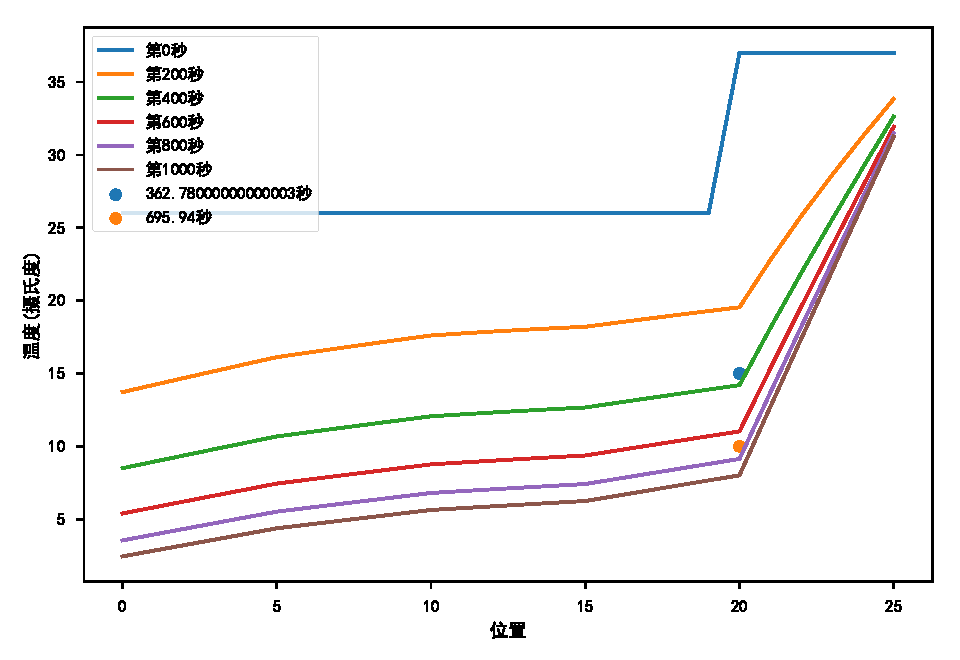
\includegraphics[width=0.95\textwidth]{T_sliceprob2.pdf}
\caption{人体—防护服—外界系统各位置不同时刻的温度变化曲线}
	\end{minipage}
	\begin{minipage}[t]{0.48\textwidth}
		\centering
	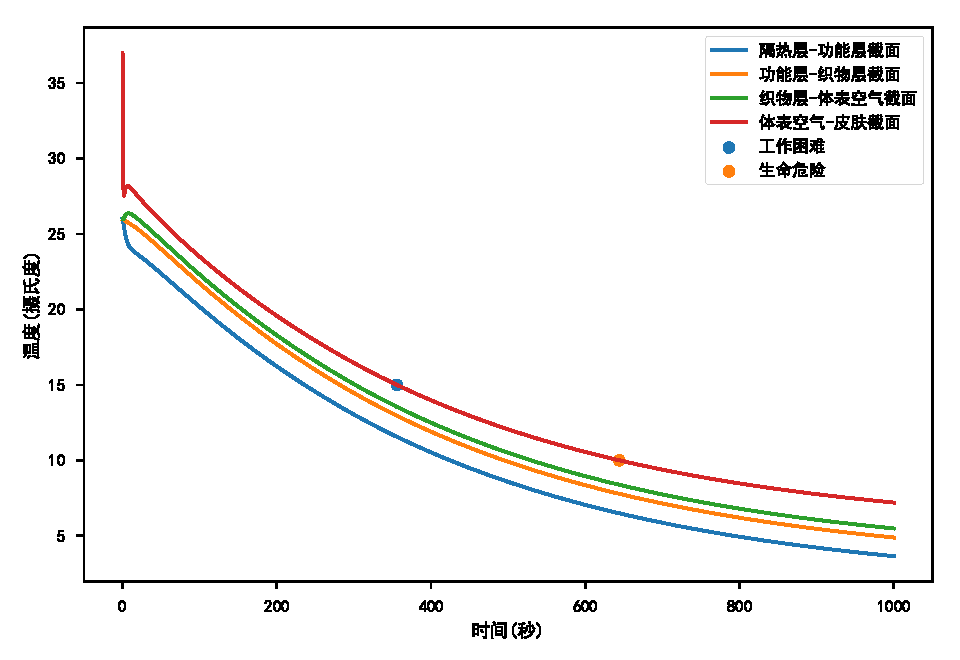
\includegraphics[width=0.95\textwidth]{x_sliceprob2.pdf}
\caption{各接触面不同时刻的温度变化曲线}
	\end{minipage}
\end{figure}
%\begin{figure}[!htbp]
%	\centering
%	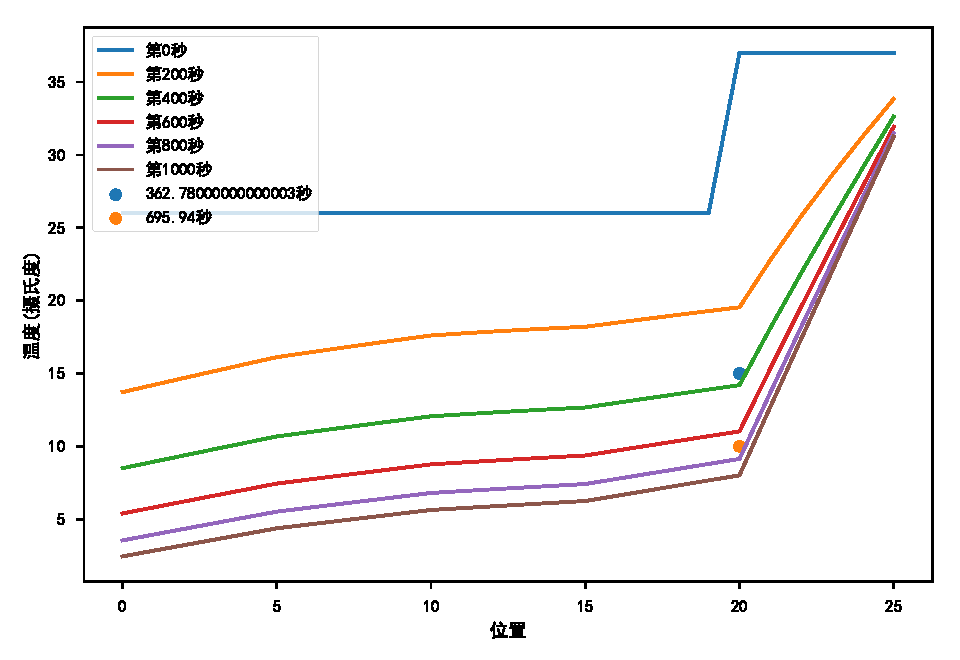
\includegraphics[width=0.6\textwidth]{T_sliceprob2.pdf}
%	\caption{人体—防护服—外界系统各位置不同时刻的温度变化曲线}
%\end{figure} 
%\begin{figure}[!htbp]
%	\centering
%	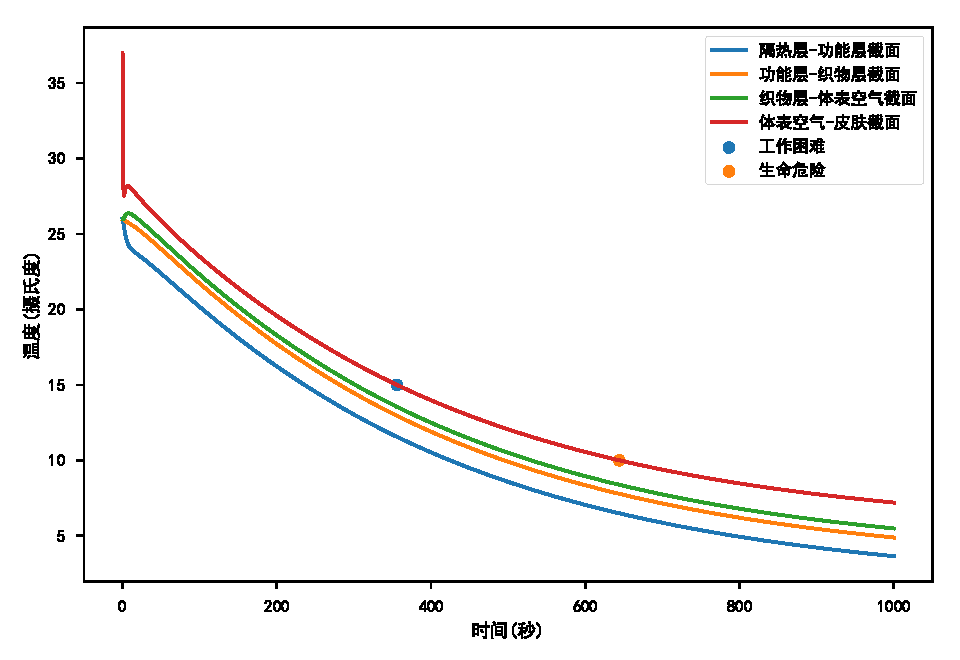
\includegraphics[width=0.6\textwidth]{x_sliceprob2.pdf}
%	\caption{各接触面不同时刻的温度变化曲线}
%\end{figure} 

\subsection{灵敏度分析}
相比于第一问我们可以很明显的看出人体皮肤温度受到外界风速的变化和人体新陈代谢速率的影响很大,所以我们在这里对$h_c$和$q_0$做变量的调整从而观察出其降温过程的变化,从图\ref{fig:hin_sensitivity_prob2}和图\ref{fig:hout_sensitivity_prob2}可以看出来,\textbf{加快外层对流系数其体表降温速率越快,新陈代谢速率增加能有效延长体表降温的时间,从而使得其存活时间更长.}
\begin{figure}[!h]
	\begin{minipage}[t]{0.48\textwidth}
		\centering
	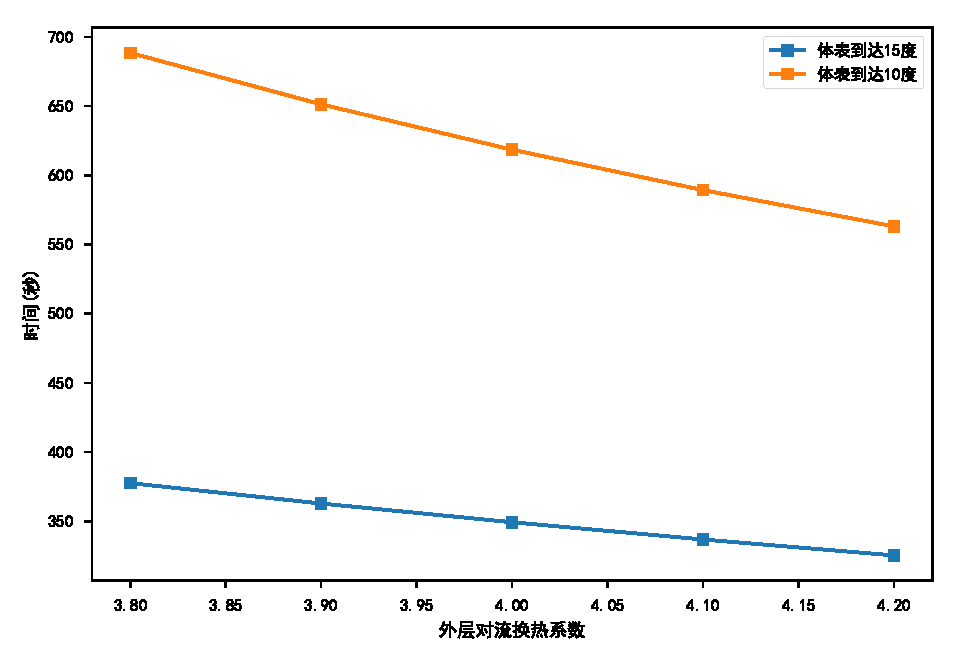
\includegraphics[width=0.95\textwidth]{hout_sensitivity_prob2.pdf}
\caption{外层对流换热系数对体表温度的影响}
\label{fig:hin_sensitivity_prob2}
	\end{minipage}
	\begin{minipage}[t]{0.48\textwidth}
		\centering
	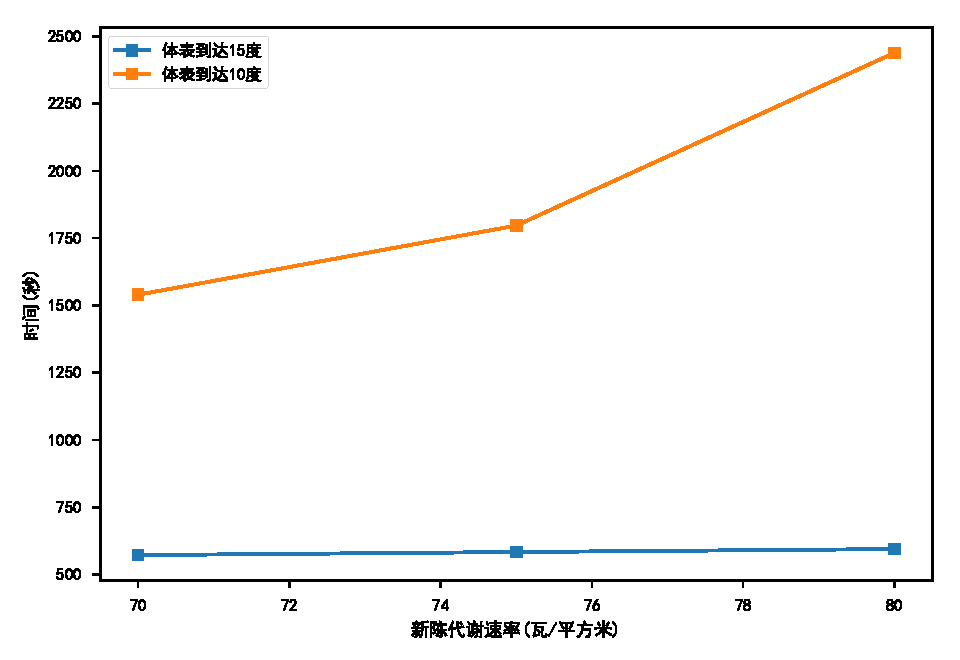
\includegraphics[width=0.95\textwidth]{hin_sensitivity_prob2.pdf}
\caption{新陈代谢速率对体表温度的影响}
\label{fig:hout_sensitivity_prob2}
	\end{minipage}
\end{figure}
%\begin{figure}[!htbp]
%	\centering
%	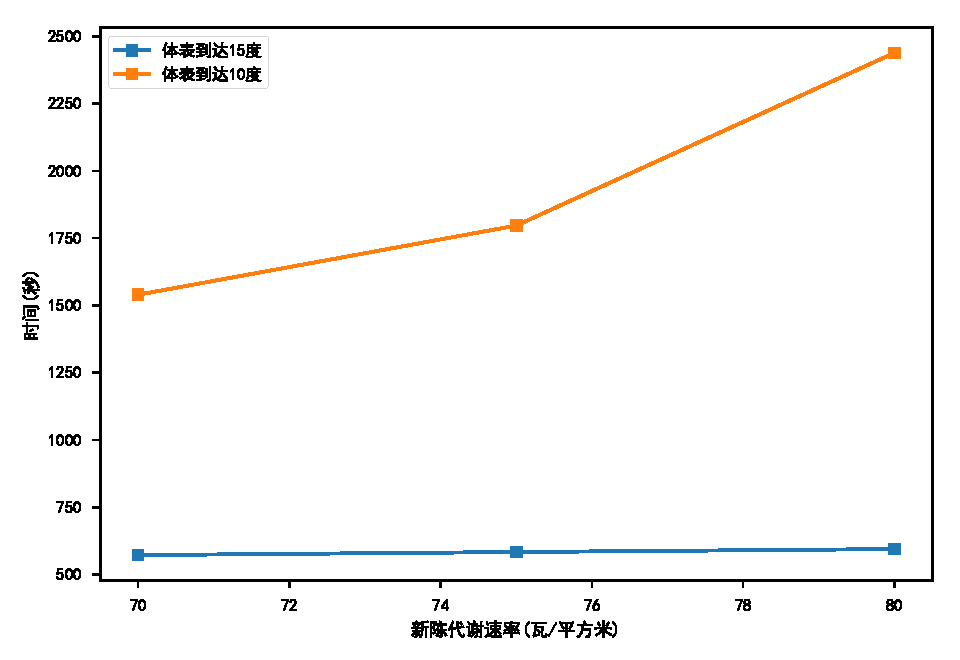
\includegraphics[width=0.6\textwidth]{hin_sensitivity_prob2.pdf}
%	\caption{外层对流换热系数对体表温度的影响}
%\end{figure} 
%
%\begin{figure}[!htbp]
%	\centering
%	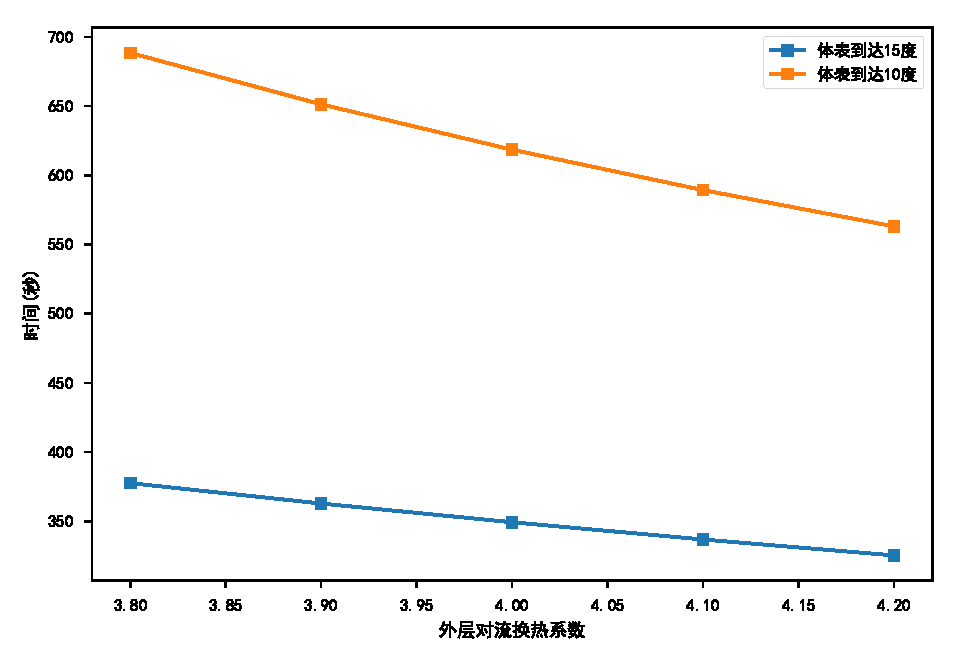
\includegraphics[width=0.6\textwidth]{hout_sensitivity_prob2.pdf}
%	\caption{新陈代谢速率对体表温度的影响}
%\end{figure}
\section{问题三模型的建立与求解}
\subsection{问题分析}问题三是一个优化问题,试验者在室外环境中面临着一个困难,即防护服的承重能力会随时间的流失而下降,在防护服的承重能力下降至实验者体重之前,实验者必须回到试验站.如果实验室愿意为低温防护服的材料多支出至多50\%的资金,请选择一种增加防护服任意层厚度的方案,使得实验者能站在外面的时间尽量长,要注意的是功能层厚度不能超出一定阈值,否则就会因为衣物太硬而无法工作,后期增加衣物厚度只能增加最外层,且最外层有固定的涂层厚度规定.

\begin{figure}[!htbp]
	\centering
	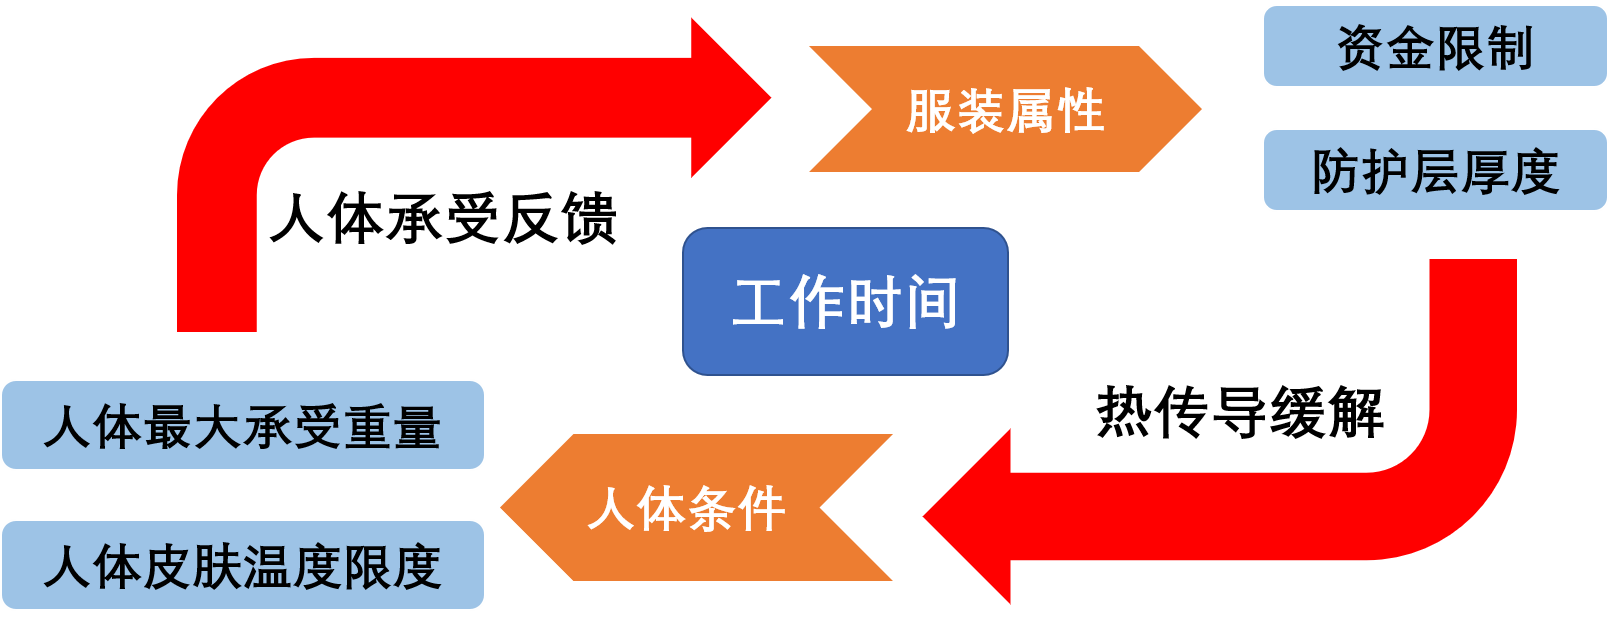
\includegraphics[width=0.6\textwidth]{map3.png}
	\caption{问题三思维导图}
\end{figure} 

\newpage
\subsection{防护服属性和工作时间优化模型}

\subsubsection{防护服价格计算}
防寒服的基础造价取决于各层织物的价格总和,隔热层和功能层的材料价格按照其质量计算,而功能层的材料价格取决于其使用面积.防寒服的大小是根据工作者的核心区域表面积设计的,由各层织物的表面积,厚度及密度我们可以求出各层织物的质量,或者可以通过表面积乘以单位面积造价直接得出价格.
设防护服设计预算为$Cost$,则防护服的预算可以表示为:
\begin{equation}
Cost=h_{1}SN\rho_{1}p_{1}+h_{2}SN\rho_{2}p_{1}+NSp_{3}.
\end{equation}
其中$h_{1},h_{2}$分别为最外层和内层的厚度,$\rho_{1},\rho_{2}$分别为最外层材料与能蹭材料的密度,$S$为人体体表面积,$N$为有效面积百分比.$p_{1},p_{2},p_{3}$分别为外层,内层和功能层的价格.求出的预算价格$Cost$为77.6元.


\subsubsection{目标函数}
因为织物材料有一定的加工要求,材料的厚度只能选择离散的数值,如外层隔热层的涂层每层厚度固定$\Delta o$为0.3mm,即每次最少要增加0.3mm.不妨假设内层织物层每层厚度$\Delta c$固定为0.1mm,在一定的预算约束下,增加防护服的厚度可以看做是一个整数规划模型.

对于中间层功能层而言,其价格与厚度无关,但不能超过一定的阈值,而且厚度越大,相变潜热越高,所以中间层功能层加厚最大值0.45mm.

对防护服进行改造的目的是为了增强其保温性能,在一共$b$种可行方案中,假设$Lo_i$,$Lc_i$分别为最外层,织物层增加的涂层数,其中$i=1,2...b$.我们的目标是找到使保温时间增长幅度最大的一种方案.
\begin{equation} 
T=\max_{i} {Time(Lo_i, Lc_i)},
\end{equation}
其中$Time()$是在体表温度降低到15 \textcelsius 前的时间。

\subsubsection{约束条件}
对防护服的改进受到资金的约束.实验室愿意为防护增增加50\%的成本投入,各层材料的成本已给出.防护服在外界承受重量的最大值会随时间的流失而减小,指导防护服的最大承载重量小于人的体重,实验者面临危险.对于中间层的相变材料,我们在允许范围内尽量增大相变材料的厚度.

\textbf{费用约束:}衣物各层材料应增加而导致的成本增长的和不能超过原有预算的50\%.
\begin{equation}
\Delta Cost_{i}\leq Cost\times 50\%-Cost_{g}.
\end{equation}
其中$i=1,2,...b$,
\begin{equation}
	\Delta Cost_{i}=p_{1}SN \rho_{1} Lo_{i}\Delta o +p_{2}SN \rho_{2} Lc_{i}\Delta c.\\
\end{equation}

% SN\rho_{1}

\textbf{时间约束:}
设人体体重为$WT$,防护服的最大承受体重为$WT_{max}$.防护服的实时最大承受体重为$WT_{t}$,防护服在外每10秒其承受重量的值就减少0.5kg,设该时间间隔为$\Delta t_{1}$.承受能力下降的幅度为$\Delta WT$,设对于不同的改造方案,从实验者走出长城站到体表温度下降至15\textcelsius 经过的时间为$T_{a1},T_{a2},...T_{ab}$,b是所有可行方案的数量.实验者衣物保暖的有效时间不能超过一定限制,否则防护服的最大承重量可能低于人体体重.
\begin{equation}
WT\leq WT_{t},\\
\end{equation}
\begin{equation}
WT_{t}= WT_{max}-\frac {T_{ai}}{\Delta t_{1}}\times \Delta WT,i=1,2,...b. \\
\end{equation}

\subsubsection{模型综述}
\begin{equation}
	T=\max_{i} {Time(Lo_i, Lc_i)},
\end{equation}
\begin{equation}
s.t.\begin{cases}
	\Delta Cost_{i}\leq Cost\times 50\%-Cost_{g}.\\
	\Delta Cost_{i}=p_{1}SN \rho_{1} Lo_{i}\Delta o +p_{2}SN \rho_{2} Lc_{i}\Delta c\\
	WT\leq WT_{t},\\
	WT_{t}= WT_{max}-\frac {T_{ai}}{\Delta t_{1}}\times \Delta WT,i=1,2,...b.
\end{cases}
\end{equation}

\subsection{结果分析}
模型的费用约束条件是一个整数线性规划问题,可以通过求出所有可能的改造方法,为了尽可能提高防寒服的保温性能,如果一种改造方案在两种衣物层上的增加涂层量都不如任意其他方案,则该方案应该被舍去.改造方案的可能取值$(n_{1},n_{2})=(1,2),(3,1)\text{或}(4,0)$.
防护服各层增加的总厚度.

\begin{equation}
\Delta D=\Delta D_{bian}+n_{1}\times 0.1+n_{2}\times 0.3.
\end{equation}
其中$\Delta D_{bian}$表示变相材料增加的宽度,固定为0.05mm.

综合上述多种方案和实际操作情况,\textbf{方案二在人体最大承受重量和资金限制下低温工作的时间是最长的,舒适层厚度设为1.0mm,功能层厚度为0.45mm,隔热层厚度为0.9mm,改造费用为37.99元.}可以验证在工作727秒之后,防护服当前的最大承受重量为64kg,大于人体与防护服的总质量60.291kg.

\begin{table}[!htbp]
	\caption{防护服优化方案} \centering
	\begin{tabular}{cccccc}
			\toprule[1.5pt]
		$\text{方案}$ &织物层厚度 &功能层厚度 &隔热层厚度&改造费用&低温工作时间\\
		\midrule[1pt]
		$\text{方案一}$ & 0.8 & 0.45 & 0.9 &31.79&631.9\\
		$\text{方案二}$ & 1.0 & 0.45 & 0.6&37.99&727\\ 
		$\text{方案三}$ & 1.1 & 0.45 & 0.3&35.36&718.02\\
		\bottomrule[1.5pt]
	\end{tabular}
\end{table}


%%\begin{table}[!htbp]
%	\caption{防护层厚度设置的方案}\label{tab001} \centering
%	\begin{tabular}{ccccc}
%		\toprule[1.5pt]
%		$D$(in) & $P_u$(lbs) & $u_u$(in) & $\beta$ & $G_f$(psi.in)\\
%		\midrule[1pt]
%		5 & 269.8 & 0.000674 & 1.79 & 0.04089\\
%		10 & 421.0 & 0.001035 & 3.59 & 0.04089\\
%		20 & 640.2 & 0.001565 & 7.18 & 0.04089\\
%		\bottomrule[1.5pt]
%	\end{tabular}
%\end{table}
%632.76 727.18 718.16

\begin{figure}[!htbp]
	\centering
	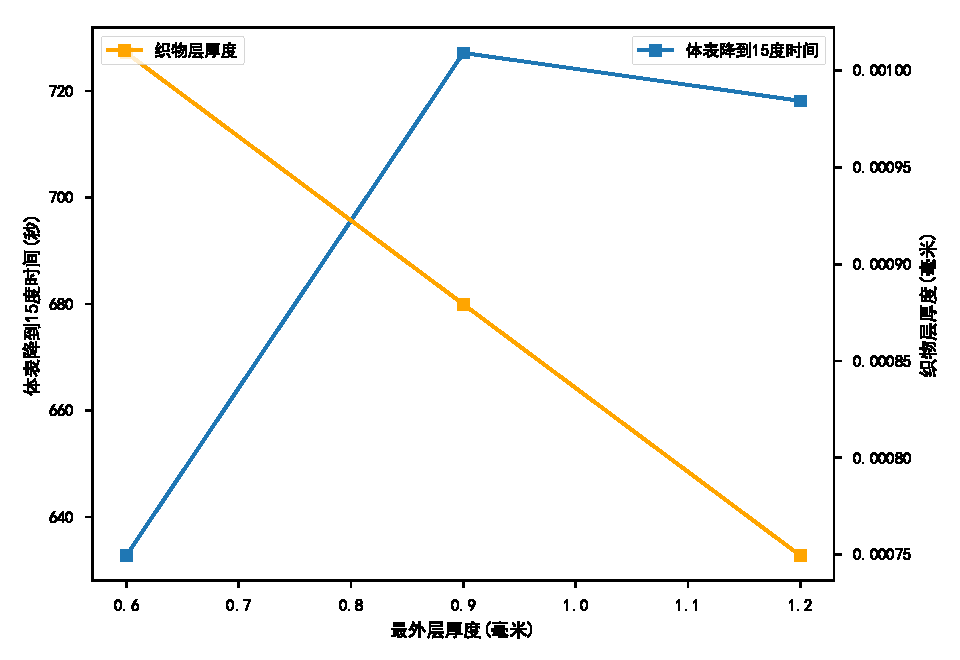
\includegraphics[width=0.7\linewidth]{time_prob3.pdf}
	\caption{防护层厚度设置与皮肤表面温度的影响}
\end{figure} 

%\subsection{灵敏度分析}

\section{问题四模型的建立与求解}
\subsection{问题分析}
问题四提出一种全新思路,如果不增加防护衣的厚度而是提高变相材料的放热能力,那么变相材料的放热能力提升多少,才能使实验者在室外坚持的时间至少不比问题三的短,假定放热能力在各个温度下是同比例增加的.通过前面3问的分析我们已经知道相变材料是通过自身放热,以防止在功能层温度过快的降低,且其放热过程是有一个范围的,即时放热能力提高也无法让材料放热的温度范围进一步扩大.
\begin{figure}[!htbp]
	\centering
	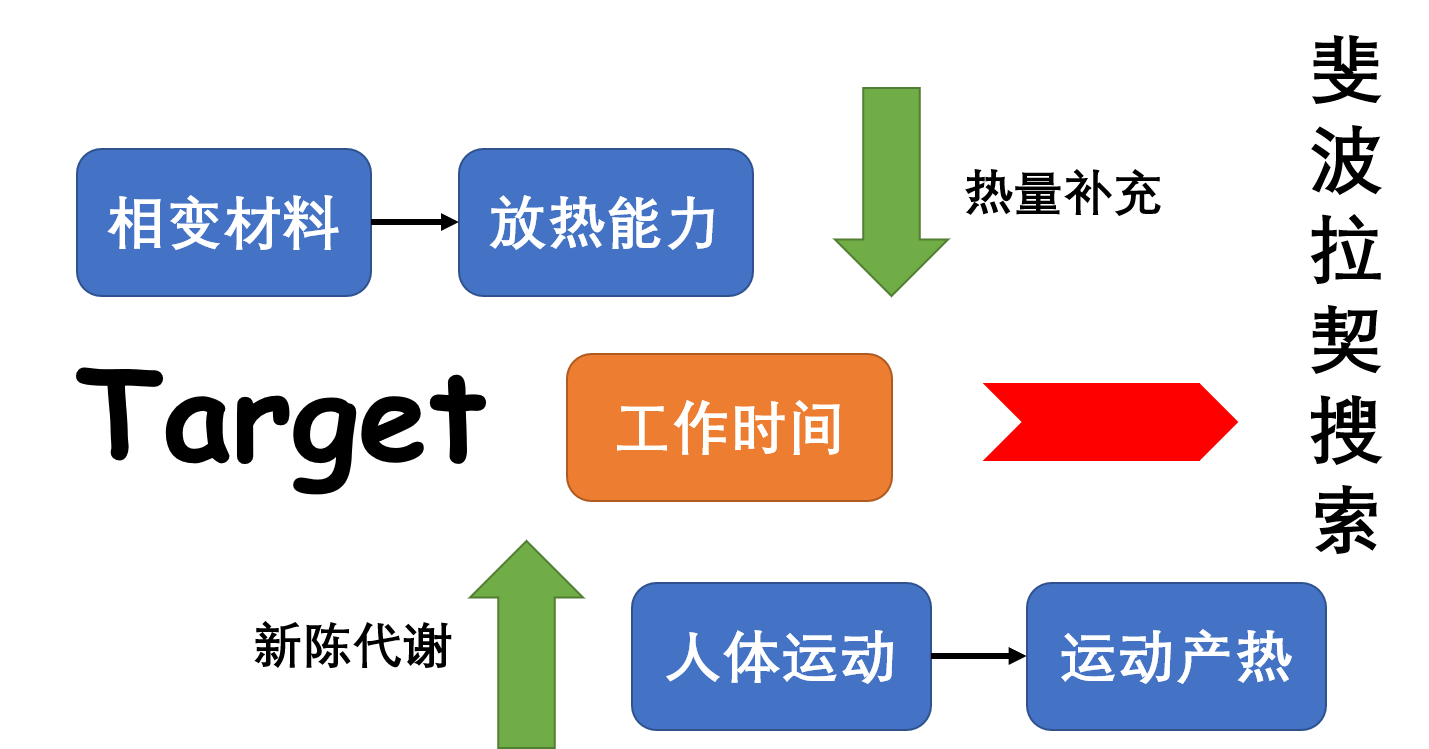
\includegraphics[width=0.6\textwidth]{map4.png}
	\caption{问题四思维导图}
\end{figure} 

\subsection{相变材料放热能力优化模型建立}
\subsubsection{相变材料能力系数衡量比例定义}
假定放热能力的提高在每个温度下是同比例增加的,即材料经过性能提升后,在每个温度下新材料的放热能力与原材料放热能力的比值是相同的.

假设材料经过一巨大幅度的能力提升,设新材料的放热能力为$DSC_{max}$,是原材料放热能力的$K_{max}$倍,称之为材料能力系数.
\begin{equation}
DSC_{max}=K_{max}\times DSC.
\end{equation}
材料放热能力经过巨大提升后,假定能够满足题目需要,则需要找到一个相对小的材料能力系数$K^{\prime}$,使得新材料能够满足保温的时间限制,显然$1\le K^{\prime}\leq K_{max}$.

\subsubsection{斐波那契区间搜索}
斐波那契(Fibonacci)搜索法,是一种一维搜索的区间消去法,这种方法与黄金分割法类似,在计算过程中第一次迭代需要计算两个迭代点,以后每次迭代只需新计算一点,另一点取自上次迭代.斐波那契法探索区间长度的缩短率采用斐波那契数,用数列\{$F_{n}$\}表示.
\begin{equation}
F_{0}=F_{1}=1,
\end{equation}
\begin{equation}
F_{n}=F_{n-1}+F_{n-2},n=2,3,4...
\end{equation}
对闭区间$[1,K_{max}]$,按相邻两斐波那契数之比,使用对称规则进行搜索,逐步缩短所考察的区间,以尽量少的运算次数求目标近似值,要求达到某一缩短率,确定搜索次数$n$,选择两系数$k_{1}$,$k_{2}$:
\begin{equation}
k_{1}=\frac{F_{n-1}}{F_{n}},k_{2}=\frac{F_{n-2}}{F_{n}}.
\end{equation}
用区间最大值乘以两系数得到确定的分割点$K{1i},K{2i},i=1,2,3,...n$,求出在此两种能力系数时,防寒服保持温暖的时间,与要求的最短时间$T_{re}$进行比较,求出要求时间与较大时间的误差,依据比较结果和判定结果重新确定搜索区间.
\subsection{模型求解}
利用斐波那契算法求解最小能力提升系数的步骤如下:

\textbf{Step1:区域初始化
}
设区域端点为$C_{1i},C{2i},i=0,1,....n.$初始化区域端点为$C_{10},C_{20}$.确定搜索次数$n$,依据斐波那契数列生成分割系数$k_{1},k_{2}$.用区间最大值乘以两分割系数得到分割点$K_{1i},K_{2i}.$

\textbf{Step2:区间搜索}

根据模型一计算在两种能力提升系数下的坚持时间$T_{K_{1i}},T_{K_{2i}}$.比较最低要求时间$T_{re}$与$T_{K_{1i}},T_{K_{2i}}$的大小关系,缩小区间范围,$i=i+1$.

\textbf{Step3:求解精度分析}

计算新区间上右端点处的时间$T_{C_{1i}}$,若满足$|T_{C_{1i}}-T_{re}|<EOL T_{re}$,则输出相应的分割点$K_{1i}$其中$EOL$是模型精度限制,设置为2\%.若不满足,重复步骤二.
\begin{algorithm}
	\caption{斐波那契算法}
	\begin{algorithmic}
		\Require C初始化端点
		\Require k斐波那契序列生成分割系数
		\State $k_{1}=\frac{F_{n-1}}{F_{n}},k_{2}=\frac{F_{n-2}}{F_{n}}$
		\For{$i = 0\quad to\quad n $}  
		\State $K_{1i}=C_{1i}\times k1,K_{2i}=C_{1i}\times k2$
		\State \text{计算两种能力提升系数下的坚持时间}$T_{K_{1i}},T_{K_{2i}}$
		\State \text{比较}$T_{re}$\text{与}$T_{K_{1i}},T_{K_{2i}}$\text{的大小关系}.
		\State \text{缩小区间范围},i=i+1
		\State \text{求解精度:}
		\If {$|T_{C_{1i}}-T_{re}|<EOL T_{re}$}
		\State \text{则输出相应分割点}$K_{1i}$
		\State  break
		\EndIf
		%\For{$j\quad in\quad sorted(I,byx_{jk})$}
		%\State $G_{L}\gets G_{L}+g_{j},H_{L} \gets H_{L}+h_{j}$ 
		%\State $G_{R}\gets G-G_{L},H_{R} \gets H-H_{L}$ 
		%\State $score\gets (score,\frac{G_{L}^{2}}{H_{L}+\lambda}+\frac{G_{R}^{2}}{H_{R}+\lambda}-\frac{G^{2}}{H+\lambda})\text{的最大值}$
		%\EndFor
		\EndFor
		\Ensure 最小能力提升系数$K^{\prime}$.
	\end{algorithmic} 
\end{algorithm}

\subsection{结果分析}
利\textbf{用斐波那契算法我们求得的材料能力系数$K^{\prime}$为\textbf{7.911},即放热能力需要提升到原来的7.911倍才能在不增加衣物厚度的情况下,在外界支持727秒.}我们画出了在这种情况下,防护服系统温度分布随时间变化的图像,如图\ref{fig:T_sliceprob4}
\begin{figure}[!h]
	\begin{minipage}[t]{0.48\textwidth}
		\centering
		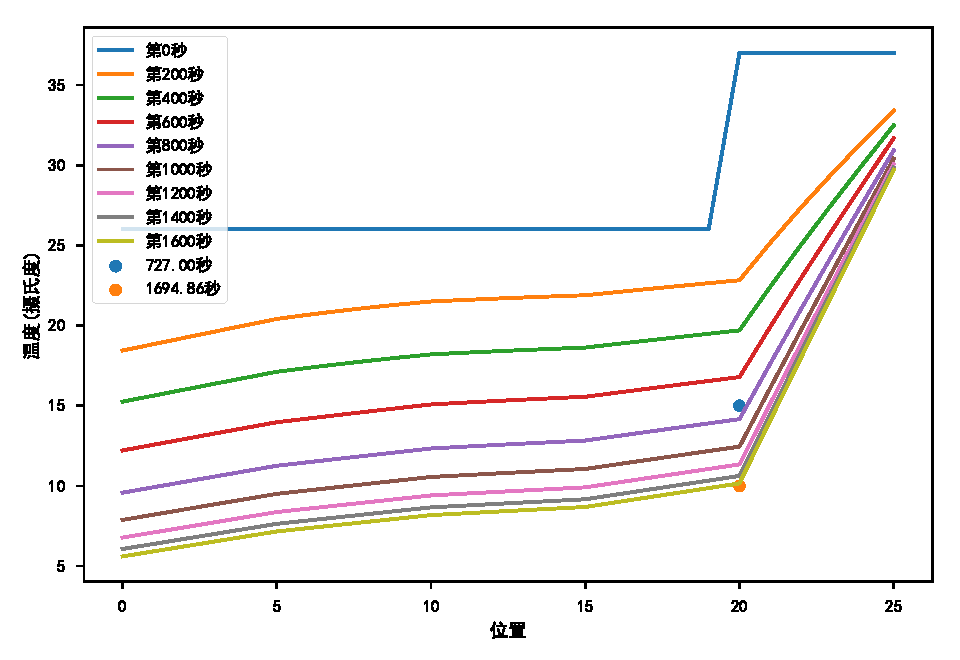
\includegraphics[width=0.95\textwidth]{T_sliceprob4.pdf}
		\caption{人体—防护服—外界系统各位置不同时刻的温度变化曲线}
		\label{fig:T_sliceprob4}
	\end{minipage}
	\begin{minipage}[t]{0.48\textwidth}
		\centering
		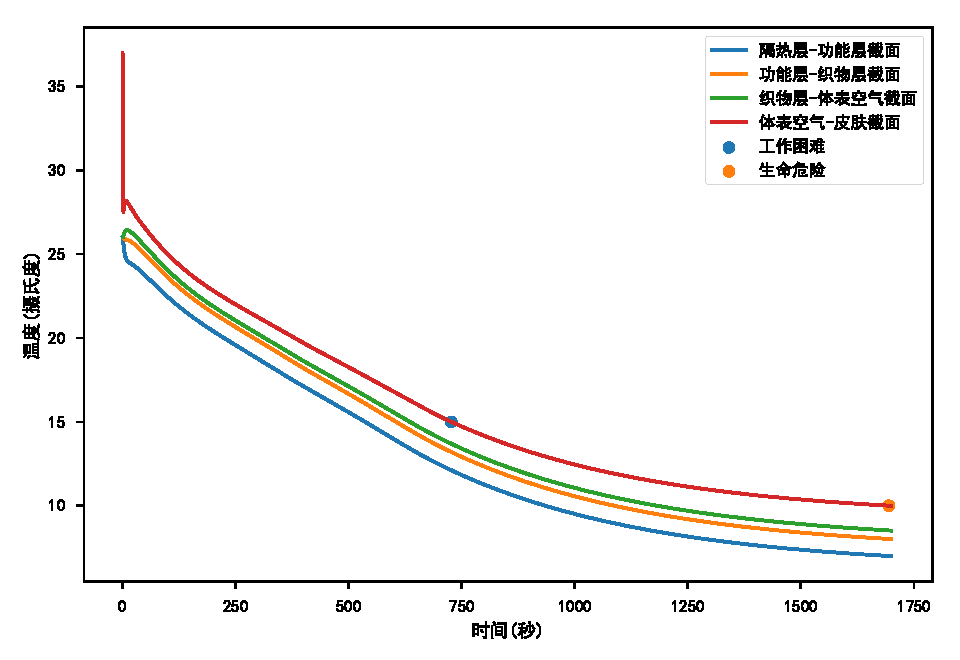
\includegraphics[width=0.95\textwidth]{x_sliceprob4.pdf}
		\caption{各接触面不同时刻的温度变化曲线}
	\end{minipage}
\end{figure}
\subsection{灵敏度分析}
我们对材料能力系数,外层对流换热系数和人体新陈代谢功率三个系数进行了10\%以内的微调,
\begin{figure}[!htbp]
	\centering
	\includegraphics[width=0.6\textwidth]{hin4.pdf}.
	\caption{新陈代谢速率对活动时间的影响}
\end{figure} 
\begin{figure}[!htbp]
	\centering
	\includegraphics[width=0.6\textwidth]{hout4.pdf}.
	\caption{对流换热系数对活动时间的影响}
\end{figure} 
结果发现随着放热能力的升高,实验者在外坚持的时间能够显著增加,\textbf{放热能力每增加一倍,实验者能在外界多活动约30秒},同时考虑到人体新陈代谢速率的差异和外层对流换热系数的变化,我们发现人体新代谢增加可以增加在外的活动时间,但是新陈速率的提高并不会使得人体在外时间明显增长,新陈代谢速率提高7\%左右,只会使得在外活动时间延长2\%,\textbf{说明在极冷环境下人体很难通过调整自身代谢速率以维持自身温度};同时,外界对流换热系数每提高约3.3\%,在外界活动时间会下降约9.2\%,\textbf{这说明衣服与外界的热对流传递受到风速或其他外界调节的影响非常大,在外活动时应尽量避免恶劣天气.}


\section{模型评价}

\subsection{模型的优点}
1.使用Crank-Nicolson方法保证了求解的稳定性,通过采用后向欧拉法避免了解的伪震荡,保证了结果的准确性.

2.用人体新陈代谢率估计人体向外发热的热流密度,考虑运动强度会导致新陈代谢率发生变化,模型贴合实际.

3.问题4斐波那契法采用区间消去的思维,相比二分法减少了迭代的搜索次数.

\subsection{模型的缺点}

1.为了简化模型忽略了部位散热速率的差异.人体的代谢散热主要由躯干部位的产热量.

2.为了简化模型忽略了衣服的褶皱,层织物与人体表面之间空气厚度的变化对散热的影响.

\subsection{改进与展望}
可以基于人体不同区域发热情况的不同,建立对人体整体区域发热进行综合的热传递模型,考虑到四肢发热与核心区域发热量的区别,建立考虑温度沿人体高度方向传播的二维热传递模型.由于四肢发热量较少,人体表体温的分布可能出现较大区别,实际情况下人体表面温度下降速度可能会加快.



\appendix %%附录
%参考文献引用\upcite{bib:one,bib:two}
\begin{thebibliography}{9}%宽度9
	\bibitem{bib:one}叶宏,张云鹏,葛新石.相变防护服的数值研究[J].中国科学技术大学学报,2005(04):538-543.
	\bibitem{bib:two}张芃.冷环境不同代谢水平下相变调温服防护需求分析[D].苏州大学,2015.
	\bibitem{bib:three}徐笑锋,章学来,张时华,赵祎.基于有限时间热力学的相变蓄放冷特性分析与研究[J/OL].热科学与技术:1-6.
	\bibitem{bib:four}晏叶.相变冷防护服系统热量散失及影响因素的研究[D].苏州大学,2017.
	\bibitem{bib;five}Rathod M K , Banerjee J . Thermal Performance of a Phase Change Material-Based Latent Heat Thermal Storage Unit[J]. Heat Transfer - Asian Research, 2015, 43(8):706-719.
	\bibitem{bib:six}姬长发,许多,李美晨,杨晨雨.相变蓄冷材料包间隙对冷却服热湿传递特性的影响[J].煤矿安全,2020,51(08):239-244.
	\bibitem{bib:seven}朱方龙.附加相变材料层的热防护服装传热数值模拟[J].应用基础与工程科学学报,2011,19(04):635-643.
\end{thebibliography}
\newpage

\section{代码}
\subsection{python源程序}
\subsubsection{main.py}
该文件是代码运行入口,调用解决问题1至4的函数.
\lstinputlisting[language=python]{code/main.py}

\subsubsection{heat\_pde.py}
该文件是偏微分方程模型的求解代码.
\lstinputlisting[language=python]{code/heat_pde.py}
\subsubsection{plot.py}
该文件打包画图函数.
\lstinputlisting[language=python]{code/plot.py}
\subsubsection{common.py}
该文件打包配置常用的第三方库
\lstinputlisting[language=python]{code/common.py}

\end{document}